\documentclass[letter,12pt]{report}
\usepackage[utf8]{inputenc}
\usepackage[T1]{fontenc}
\usepackage[spanish, es-tabla]{babel}
\usepackage[sfdefault, condensed]{roboto}
\usepackage[margin=1cm]{geometry}
\usepackage{multicol,fancyhdr,eso-pic,url,float,cite,lmodern,listings,times,textcomp, amsthm,amsmath,amssymb,dsfont,color,colortbl,sidecap,xspace,epic,eepic,anysize,setspace, hyperref, pdflscape,lscape}
\usepackage{blindtext, subcaption}
\usepackage[demo]{graphicx}
\graphicspath{ {./img/} }

%%%%%%Glosario
%\usepackage[acronym]{glossaries}
%\makeglossaries
%\renewcommand{\glossaryname}{Glosario}
%\renewcommand{\acronymname}{Acrónimos}


\usepackage{apacite} %bibliografias Bibtex

%Tipos de Letra
%\renewcommand{\rmdefault}{phv} % Arial
\usepackage{mathptmx} %Times
%Margenes
\marginsize{3cm}{2cm}{2cm}{2cm}
\spacing{1.5}%interlineado

\providecommand{\keywords}[1]{\textbf{\textit{Palabras Clave---}} #1}

\newcommand\BackgroundPic{ \put(-3,0){ \parbox[b][\paperheight]{\paperwidth}{ \vfill \centering 
\includegraphics[width=\paperwidth,height=\paperheight]{portada.jpg} \vfill }}} 

%Definicion de Colores
\definecolor{gray97}{gray}{.97}
\definecolor{gray75}{gray}{.75}
\definecolor{gray45}{gray}{.45}
\definecolor{verdeo}{rgb}{0,.5,0.2}
\definecolor{listinggray}{gray}{0.9}
\definecolor{lbcolor}{rgb}{0.9,0.9,0.9}
\newcommand\gris[1]{\textcolor[gray]{.35}{\emph{#1}}}
\newcommand\rojo[1]{\textcolor[rgb]{1,0,0}{#1}}
\newcommand\blue[1]{\textcolor[rgb]{0,0,1}{{#1}}}
\newcommand\azul[1]{\textcolor[rgb]{0,0,1}{#1}}
\newcommand\verde[1]{\textcolor[rgb]{0,.5,0.2}{#1}}
\newcommand\naranjo[1]{\textcolor[rgb]{1.00,0.36,0.06}{\textbf{#1}}}
\newcommand\blanco[1]{\textcolor[rgb]{1,1,1}{\textbf{#1}}}
\newcommand {\red}[1]{\textcolor[rgb]{1.00,0.00,0.00}{#1}}
\newcommand\cita[1]{{\scriptsize \begin{flushright}\emph{(#1)}\end{flushright}}}



%%%Entornos de desarrollo
\newtheorem{ejemplo}{Ejemplo}
\newtheorem{definir}{Definición}
\newtheorem{prueba}{Prueba}
\newtheorem{demo}{Demostración}
\newtheorem{obs}{Observación}

\newcommand{\ignore}[1]{}

%%%CODIGOS DE PROGRAMACION
\lstset{%backgroundcolor=\color{lbcolor},
    frame=Ltb, framerule=0pt, aboveskip=0.5cm, tabsize=4, rulecolor=, language=C, %%%CAMBIAR POR LENGUAJE DE PREFERENCIA
    stringstyle=\ttfamily,  %basicstyle=\footnotesize,
    upquote=true, aboveskip={1.5\baselineskip}, columns=fixed, showstringspaces=false, extendedchars=true,breaklines=true, prebreak = \raisebox{0ex}[0ex][0ex]{\ensuremath{\hookleftarrow}}, showtabs=false, showspaces=false, showstringspaces=false,
    %tipos de letra y colores
    identifierstyle=\ttfamily,
    keywordstyle=\bfseries  \color[RGB]{0,2,216}, %palabras reservadas
    commentstyle= \scriptsize\color[rgb]{0,.5,0.2}, %comentarios
    stringstyle=\color[RGB]{216,0,114},%cadena de texto
    %numeracion de lineas
    framextopmargin=3pt, framexbottommargin=3pt, framexleftmargin=0.4cm,
    framesep=0pt, rulesep=.4pt, rulesepcolor=\color{black}, numbers=left, numbersep=15pt, numberstyle=\tiny, numberfirstline = false, breaklines=true,literate={á}{{\'a}}1 {é}{{\'e}}1 {í}{{\'i}}1 {ó}{{\'o}}1 {ú}{{\'u}}1
    {Á}{{\'A}}1 {É}{{\'E}}1 {Í}{{\'I}}1 {Ó}{{\'O}}1 {Ú}{{\'U}}1
    {à}{{\`a}}1 {è}{{\`e}}1 {ì}{{\`i}}1 {ò}{{\`o}}1 {ù}{{\`u}}1
    {À}{{\`A}}1 {È}{{\'E}}1 {Ì}{{\`I}}1 {Ò}{{\`O}}1 {Ù}{{\`U}}1
    {ä}{{\"a}}1 {ë}{{\"e}}1 {ï}{{\"i}}1 {ö}{{\"o}}1 {ü}{{\"u}}1
    {Ä}{{\"A}}1 {Ë}{{\"E}}1 {Ï}{{\"I}}1 {Ö}{{\"O}}1 {Ü}{{\"U}}1
    {â}{{\^a}}1 {ê}{{\^e}}1 {î}{{\^i}}1 {ô}{{\^o}}1 {û}{{\^u}}1
    {Â}{{\^A}}1 {Ê}{{\^E}}1 {Î}{{\^I}}1 {Ô}{{\^O}}1 {Û}{{\^U}}1
    {œ}{{\oe}}1 {Œ}{{\OE}}1 {æ}{{\ae}}1 {Æ}{{\AE}}1 {ß}{{\ss}}1
    {ű}{{\H{u}}}1 {Ű}{{\H{U}}}1 {ő}{{\H{o}}}1 {Ő}{{\H{O}}}1
    {ç}{{\c c}}1 {Ç}{{\c C}}1 {ø}{{\o}}1 {å}{{\r a}}1 {Å}{{\r A}}1
    {€}{{\EUR}}1 {£}{{\pounds}}1 {Ñ}{{\~N}}1 {ñ}{{\~n}}1 {¿}{{?`}}1
}
%%%%FIN CODIGOS DE PROGRAMACION
\def\figurename{}

%%%%%%%%%%ENCABEZADO Y PIE DE PAGINA
%encabezado de las paginas pares e impares.
\rhead[PP]{Ingeniería Civil en Informática}
\renewcommand{\headrulewidth}{0.5pt}
%pie de pagina de las paginas pares e impares.
\lfoot[nombre]{Muñoz Viveros}
\rfoot[rut]{Universidad de los Lagos}
\renewcommand{\footrulewidth}{0.5pt}
%encabezado y pie de pagina de la pagina inicial de un capitulo.
\fancypagestyle{plain}{
    \fancyhead[R]{Ingeniería Civil en Informática}
    \fancyfoot[L]{Muñoz Viveros}
    \fancyfoot[R]{Universidad de los Lagos}
    \renewcommand{\headrulewidth}{0.5pt}
    \renewcommand{\footrulewidth}{0.5pt}
}
\pagestyle{fancy} 
%%%%%%%%%%FIN ENCABEZADO Y PIE DE PAGINA 

\begin{document}

%%%%%%%%%%%PORTADA%%%%%%%%%%%%%%%%%%%%%
\setlength{\unitlength}{1 cm} %Especificar unidad de trabajo
\thispagestyle{empty}

\AddToShipoutPicture*{\BackgroundPic}
\title{\vspace{-1cm}\scshape\Large{\textbf{Detección de presencia de parásitos en examen
    parasitológico seriado de deposiciones con visión por computadora}}\\\vspace{0.5cm}
    \large Departamento de Ciencias de la Ingeniería\\
    \large Ingeniería Civil en Informática\\
Campus Puerto Montt, Chile}
\author{
    \vspace*{-2cm}
    Diego Ignacio Muñoz Viveros\\
    diegoignacio.munoz@alumnos.ulagos.cl
}
\date{Profesor Guía: Joel Sebastian Torres Carrasco\\  Co-guía: Carlos Dupré Alvarado\\
\today}
\maketitle
\ClearShipoutPicture


\cleardoublepage
\pagenumbering{roman}
\setcounter{page}{1}

%%%%Agradecimientos
\chapter*{Agradecimientos}
Gracias

%%%%%%%%RESUMEN
\begin{abstract}
    El examen parasitológico seriado de deposiciones es un examen realizado para la
    detección de presencia parasitológica en pacientes. El examen se lleva a cabo con la
    toma de muestras de deposiciones del paciente y posteriormente se hace observación de
    las mismas por medio de microscopio, en la realización de la observación se documenta
    la confirmación y clasificación de presencia parasitológica en orden de dar con un
    tratamiento certero, eficaz y acorde a las detecciones.

    El uso de la visión por computadora espera demostrar el aumento en la precisión y
    velocidad de la detección y clasificación de parásitos con objetivo de reducir
    incertidumbre y error humano introducido en la observación manual ejercida en el
    proceso de observación del examen parasitológico seriado de deposiciones. La visión
    por computadora es la combinación de tecnologías que permite a las computadoras
    generar inferencia respecto a imágenes estáticas o en movimiento emulando la visión
    humana por medio de un aprendizaje basado en conjuntos de datos utilizados como
    ejemplos iniciales de los cuales el modelo generado ajustará sus parámetros.

    En el presente trabajo, se realizó una búsqueda de conjuntos de datos sobre parásitos,
    se desarrolló un modelo de clasificación de imágenes basados en visión por computadora y
    se probaron diferentes alternativas para mejorar la calidad de la identificación y la 
    clasificación.

    Finalmente, este trabajo aporta un marco experimental sobre un conjunto de datos acotado
    de parásitos, que puede ser liberado a producción, ampliando la cantidad de parásitos a
    identificar.

%Resume en un (1) párrafo el contenido del informe en un máximo de 350 palabras.
%Debe ser preciso:
%\begin{itemize}\justifying
  %\item Establece el problema
  %\item Dice porqué es interesante
  %\item Señala los logros y desafios
%\end{itemize}
%Un resumen debe ser llamativo, motivador, descriptivo y sin contenido específico. \textbf{No incluye}: citas, referencias, conclusiones, figuras ni tablas.
%
%
\keywords{Parasitólogia, Serializado, Deposiciones, Visión por Computadora, Modelo,
Conjunto de Datos, \textit{Underfiting}, \textit{Overfiting}}
\end{abstract}


%%%%%%INDICES
\tableofcontents
\listoffigures
%\renewcommand{\listtablename}{Índice de tablas}
%\listoftables
%\renewcommand{\lstlistlistingname}{Índice de algoritmos}
%\lstlistoflistings
%\addcontentsline
%%%%%%%%%%%%%FIN PORTADA%%%%%%%%%%%%%%%%

\cleardoublepage
\pagenumbering{arabic}
\setcounter{page}{1}

%%%%%%%%COMIENZO



\chapter{Introducción}\label{intro}

%cita1: http://scielo.sld.cu/pdf/mgi/v22n1/mgi07106.pdf
Los exámenes, pruebas o mediciones médicas son la base para la evaluación médica y
estudios clínicos que permitan elaborar diagnósticos correctos y, consecuentemente,
plantear tratamientos adecuados.  Los exámenes médicos son procedimientos rigurosos
que permiten observar el comportamiento humano siguiendo el método científico para
recolectar evidencias, en este caso, del cuerpo humano. Para poder medir de mejor
manera todos estos comportamientos, se han desarrollado diferentes técnicas a lo
largo del tiempo, como la observación, análisis químico o genético.  Por ende, la
calidad de los exámenes médicos son un factor clave para que los tratamientos dados
tengan efectos positivos y, finalmente, mejorar la calidad de vida de los pacientes.

% Todavía hay gran cantidad de exámenes echos a mano
% Hacer esto a mano no suple la demanda médica
En la actualidad, los laboratorios médicos son los encargados de realizar una gran
cantidad de exámenes relacionados a la observación microscópica de muestras. Estos
exámanes son ralizados bajo observación humana de manera totalmente manual
considerando a un experto llamado tecnólogo médico. 

% Introducción del rol de la tecnología médica
% Intro a nuestro laboratorio clínico cesfam de hornopiren
% Dentro de los exámenes con mirada experta
La tecnología médica en el ámbito del conocimiento abarca el estudio e investigación
que tiene como objetivo la aplicación de diferentes tipos de tecnologías para mejorar
la salud de las personas durante su diagnóstico, desarrollo de la enfermedad y
tratamiento aplicado. En el contexto médico, la tecnología médica es la rama de la
salud que involucra a profesionales que se forman en los avances tecnológicos para
aplicarlos a la medicina y las ciencias de la salud.

% cita2: https://www.scielo.cl/scielo.php?script=sci_arttext&pid=S0034-98872015000600011
Normalmente los exámenes que involucran esta observación microscópica suelen demandar
bastante tiempo por muestra; lo cual aumenta la demanda habitual en el área de la
salud y, sobretodo, en la salud pública lo que se refleja en demoras en la entrega de
resultados.

%TODO revisar
%    Para la consultoria de este trabajo se cuenta con la ayuda del laboratorio clínico
%    CESFAM de Hornopiren, con la ayuda del tecnólogo médico y jefe del laboratorio
%    clínico Carlos Dupré Alvarado.

% Sesgo humano
% Certeza incierta
Otra característica inherente de los exámenes basada en observaciones de imágenes
está relacionada al error humano introducido en las observaciones, dependiendo
totalmente de la expertiz del tecnólogo médico.  En consecuencia, las observaciones
resultante contienen clasificaciones erroneas, influyendo en un mal diagnoóstico
médico. Es así que, en ocaciones puede haber una gran diferencia entre las
observaciones de distintos tecnólogos médicos sobre la misma muestra, lo que genera
una gran incertidumbre a los estudios clínicos y que obliquen a realizar
observaciones adicionales o complementarias.

Uno de estos exámenes basados en observaciones de imágenes es el examen parasitológico 
seriado de deposiciones  que es un examen realizado para la
detección de presencia parasitológica en pacientes. Este examen se lleva a cabo con la
toma de muestras de deposiciones del paciente y, posteriormente, se hace observación
de las muestras por medio de observación microscopica. En la realización de la
observación se documenta la confirmación y clasificación de presencia parasitológica
en orden de dar con un tratamiento certero, eficaz y acorde a las detecciones. %cita aqui
La denominación seriado refiere a las condiciones en las que estas muestras, tres
muestras enfrascadas por separado, serán tomadas con la finalidad de tener muestras
en distintos ciclos larvales.

% Cual es el problema que tenemos acá
% Inconsistencia en las mediciones / definición del problema
Por lo tanto, la problemática presentada en este trabajo radica en lo altamente
susceptible al sesgo del observador del examen, es decir, es muy sensible a perdida o
mala clasificación de avistamientos llevando a malos diagnósticos médicos. 

En este trabajo se propone una solución inteligente para automatizar el examen
parasitológico seriado de deposiciones para poder mejorar la calidad de los
resultados y así mejorar la calidad de vida de las personas.

Para realizar este proyecto se pretende usar tecnologías que permitan aprovechar la
experiencia de los tecnólogos médicos para mejorar los resultados de las
observaciones.  Es por ello, que se pretende utilizar tecnologías de visión por
computadora para automatizar la observación de muestras y, a su vez, reducir el grado
de error. Además, se espera que la implementación permita simplificar y agilizar el
procedimiento de observación del examen.

La visión por computadora es la combinación de tecnologías que permite a las
computadoras generar inferencia respecto a imágenes estáticas o en movimiento
emulando la visión humana por medio de un aprendizaje basado en conjuntos de datos
utilizados como ejemplos iniciales de los cuales el modelo generado ajustará sus
parámetros.  El uso de la visión por computadora espera demostrar el aumento en la
precisión y velocidad de la detección y clasificación de parásitos con objetivo de
reducir incertidumbre y error humano introducido en la observación manual ejercida en
el proceso de observación del examen parasitológico seriado de deposiciones. 

% El gran desafió tésnico
% Uno de los problemas, existencia de dataset relacionados al examen
El desafío técnico encontrado está relacionado a la estructuración de un conjunto de
datos de imágenes microscópicas que contengas la información suficiente para generar
un modelo robusto y de altas prestación con gran capacidad de generalización para el
examen parasitologico seriado de deposiciones.

% Continua que se verá (terminar esto)
En adelante, el documento se estructura de la siguiente manera. El capítulo
\ref{teorico}, presenta los conocimientos básicos para entender el desarrollo de este
proyecto de título. El capítulo \ref{formulación}, define los objetivos, metodología
y planificación del proyecto. Finalmente, el capítulo \ref{conclusion}, entrega
algunas ideas a desarrollar a futuro en el proyecto.

\chapter{Marco Teórico}\label{teorico}

\section{Parasitología}
\subsection{Definición}
La parasitología es la rama de las ciencias biológicas dedicada a el estudio de
organismos, denominados parásitos, que dependen de otro para poder sobrevivir y que
ocasionan grandes daños a las especies de las cuales dependen, relación llamada
parasitismo.

La parasitología es una disciplina con aplicación en campos variados como medicina,
farmacología y veterinaria. Es utilizada en la investigación de parásitos que pueden
producir enfermedades en plantas y animales con objeto de analizar, diagnosticar y
posteriormente establecer un tratamiento óptimo para poder curarlas y
erradicarlas \cite{Paras}.

Gran parte de los parásitos más difícil de tratar son los que se alojan en el
interior del organismo, lo que puede ingresar por via oral o fluidos y gran parte de
estos pueden alojarse en el sistema digestivo, principalmente en estomago e
intestino \cite{Vigil}.

En el contexto de la medicina, la área de \textbf{Tecnología Médica} en su
especialización de parasitología esta encargada de la realización y análisis de
exámenes con la finalidad de diagnosticar amenazas relacionadas a la
disciplina \cite{Digest}.

\subsection{Exámenes Parasitológicos}

Existen muchos tipos de análisis de laboratorio para diagnosticar enfermedades parasitarias.
El tipo de análisis que solicite el médico se basará en sus signos y síntomas presentados
durante la consulta médica, cualquier otra afección médica que pueda tener y sus
antecedentes de viajes.

El análisis de laboratorio se lleva a cabo con las observaciones de muestras entregadas
al laboratorio por el médico tratante. Estas muestras dependen de la búsqueda de los
parásitos sospechados y sus posibles ubicaciones, siendo estas muestras de la forma de
sangre, heces, muestras urogenitales, esputo, aspirados o biopsias. La especificidad de
los exámenes puede variar en la capacidad de detectar diferentes especies o realizar
búsquedas de manera particular \cite{Util}.

Estos exámenes se pueden dividir en dos categorías:

\begin{itemize}
    \item Invasivos: la adquisición de la muestra requiere intervención
        quirúrgica algún tipo como las biopsias.
    \item No invasivos: la toma de la muestra presenta un método de obtención que no
        involucra una intervención invasiva al paciente como serían muestras de sangre o
        heces.
\end{itemize}

\subsection{Procedimiento de exámenes}

Para la realización de los exámenes se procede de las siguientes formas: \cite{Diagnost}

\begin{enumerate}
    \item \textbf{Exámenes de muestra de sangre}: la muestra es tintada y analizada por
        goteo grueso y/o fino con un microscopio. El goteo fino es una forma de repartir
        la muestra en un portaobjeto \footnote{Placa de acrílico trasparente usada para
        manejo de muestras para microscopio} a manera de dejar una capa delgada y
        uniforme en la cual realizar observaciones, el goteo grueso por otro lado,
        consiste en soltar una gota de muestra de forma que la tensión superficial de la
        muestra mantenga su forma circular para dejar decantar las células contenidas en
        la muestra al fondo.  La tinción es el proceso en el cual se suman compuestos a
        la muestra que reaccionan a componentes conocidos con el fin de teñir componente
        para facilitar la visualización.
    \item \textbf{Endoscopia/Colonoscopia}: Consiste en la inserción en la boca
        (endoscopia) o el recto (colonoscopía) de una sonda con la cual el médico,
        normalmente un gastroenterólogo, examina las cavidades en busca de presencia
        parasitaria y/o lesiones de relacionadas a presencia parasitaria.
    \item \textbf{Exámenes parasitológico seriado de deposiciones}: consiste en el
        análisis de tres muestras seriadas \footnote{Muestras tomadas con intervalos de
            tiempo equidistantes con objetivo de muestrear sin que se pierdan ciclos
        larvarios evitando excluir avistamientos} de heces tintadas con observación por
        microscopio . La observación se realiza por goteo fino.
    \item \textbf{Resonancia Magnética (RM), Tomografía axial computarizada (TAC)}:
        Pruebas realizadas para buscar enfermedades parasitarias que pueden provocar
        lesiones en los órganos.
\end{enumerate}

\subsection{Examen Parasitológico Seriado de Deposiciones (EPSD)}
% Que es, para que, procedimiento
% Hablar del contexto del tecnologo medico
Como se menciona anteriormente, el examen parasitológico seriado de deposiciones (EPSD)
es un examen que busca estudiar la presencia parasitaria intestinal por medio de
observaciones de muestras de heces. La realización de este examen es llevado a cabo por
un tecnólogo médico y su principal objetivo es documentar las observaciones realizadas.

La realización del examen en detalle se muestra a continuación:\cite{Serial}
\begin{enumerate}
    \item Una vez se reconoce la necesidad de la realización del examen, el médico
        tratante pedirá la preparación de tres frascos de muestras con 10-20 ml de
        líquido fijador\footnote{Liquido conservantes, normalmente formaldehído}.
    \item Se hace entrega al paciente de los frascos junto a una nota con las
        instrucciones para la toma de muestras, conservación de las mismas y precauciones
        a tomar \ref{fig:frascos}.
        \begin{figure}[H]
            \centering
            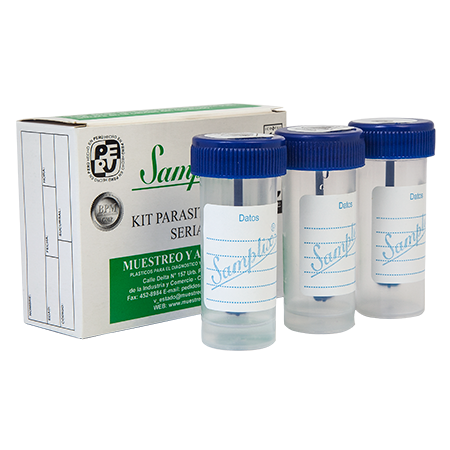
\includegraphics[width=0.4\textwidth]{frascos}
            \caption{Frascos para almacenamiento de muestras de deposiciones}
            \label{fig:frascos}
        \end{figure}

    \item Cuando se reciben las muestras y se valida su tamaño, los tiempos en los que se
        tomaron y la forma en que se conservaron, estas pasaran a ser entregadas al
        laboratorio donde serán almacenadas y/o examinadas.
    \item Las muestras son retiradas del área de refrigeración, en el caso que se
        encuentren en conservación, y se proceden a introducir una porción de cada frasco
        en tres probetas diluidas en el líquido fijador.
    \item Se centrifugan las muestras en orden de separar el material fecal del líquido
        fijador para poder extraerlo \ref{fig:sample}.
        \begin{figure}[H]
            \centering
            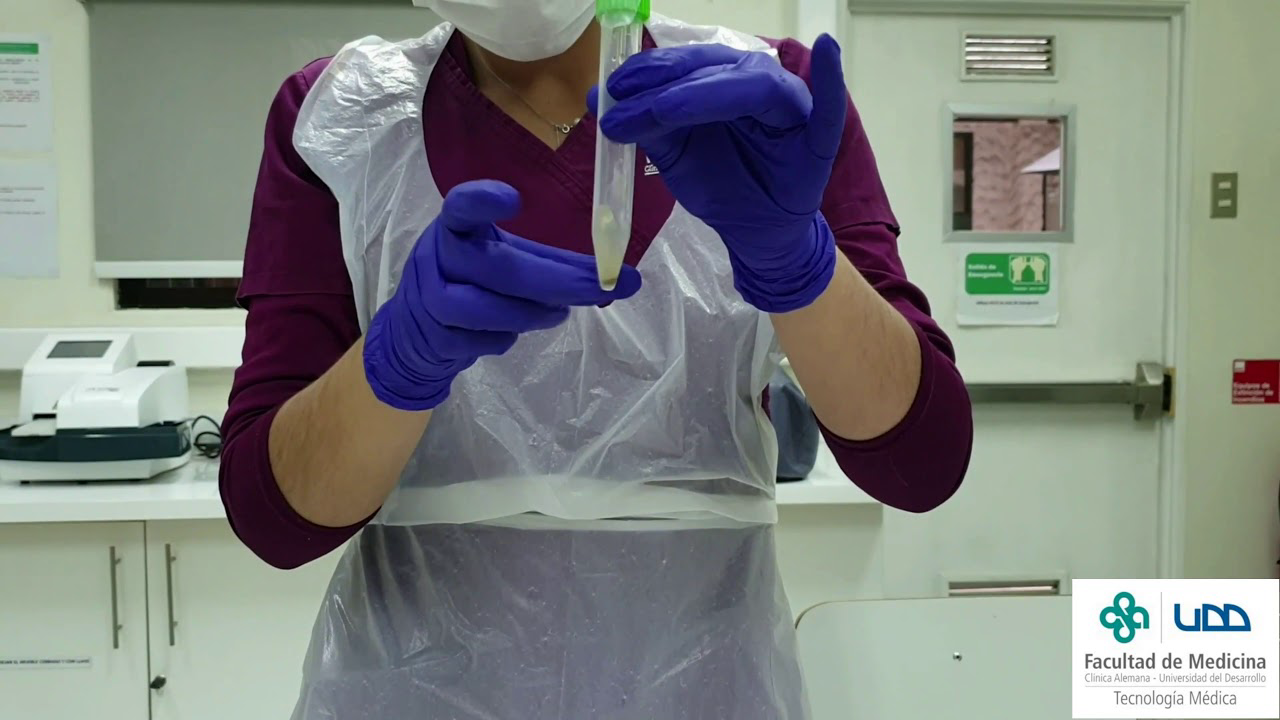
\includegraphics[width=0.5\textwidth]{sample}
            \caption{Muestra centrifugada de deposiciones}
            \label{fig:sample}
        \end{figure}
    \item En caso de que el tecnólogo lo considere necesario, tintar la muestras con
        soluciones reactivas que resalten componentes específicos para facilitar las
        observaciones.
    \item Dejar caer una gota de cada una de las muestras en un portaobjeto y esparcir
        para observación de goteo fino.
    \item Hacer observación de las muestras con gran detalle en el microscopio y
        documentar hallazgos en caso de haber \ref{fig:documentacion}.
        \begin{figure}[H]
            \begin{subfigure}{0.5\textwidth}
                \centering
                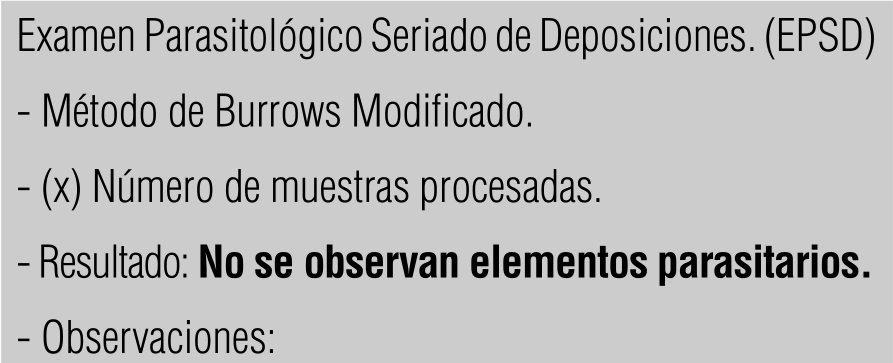
\includegraphics[width=0.8\textwidth]{negativo}
                \caption{Contenido textual en caso de no hallar presencia parasitológica}
                \label{fig:negativo}
            \end{subfigure}
            \begin{subfigure}{0.5\textwidth}
                \centering
                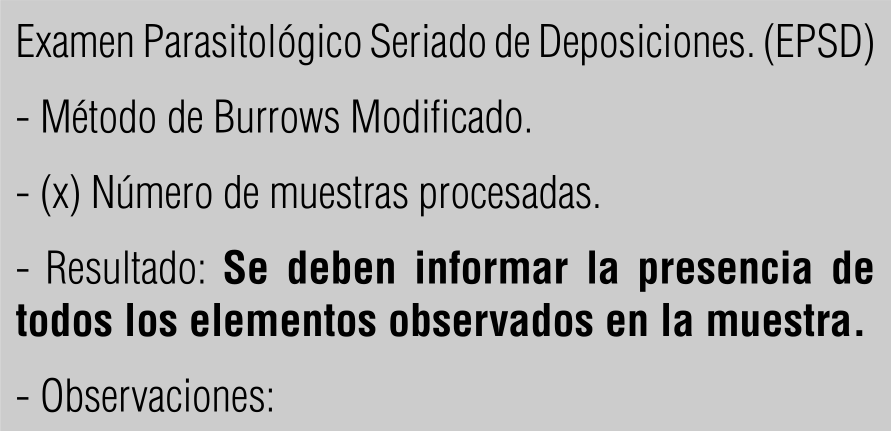
\includegraphics[width=0.8\textwidth]{positivo}
                \caption{El informe debe contener un listado detallado de las observaciones
                incluyendo nombre del parásito y cantidad de avistaminetos.}
                \label{fig:positivo}
            \end{subfigure}
            \caption{Ejemplos de documentación del examen parasitológico seriado de
            deposiciones.}
            \label{fig:documentacion}
        \end{figure}
    \item En caso de no detectar presencia parasitaria, documentar que no se observa
        presencia en la muestra.
\end{enumerate}

Para la correcta realización del examen existen ciertas consideraciones expuestas a
continuación:
\begin{itemize}
    \item La toma de muestras debe abarcar un período mínimo de cinco días.
    \item La duración de la observación microscópica puede durar al rededor de 45
        minutos y es dependiente de la habilidad y experiencia del tecnólogo.
    \item En caso de encontrar alguna anormalidad en la recepción de las muestras por
        parte del paciente, se debe pedir que este haga la toma nuevamente en frascos
        diferentes.
    \item La muestra que no se utilice durante la observación deber ser conservada en
        refrigeración.
    \item En caso de existir dudas sobre la observación de las muestras, se puede
        realizar una segunda observación.
\end{itemize}
%TODO agregar ejemplos de resultados
%TODO listado de parásitos

\section{Visión por Computadora}
\subsection{Definición}
La visión por computadora es el campo de la inteligencia artificial (IA) que permite a
los computadores y sistemas derivados a extraer información útil de imágenes digitales,
videos y otras entradas visuales y tomar acciones o hacer recomendaciones basadas en esta
información. Si la IA permite a los computadores pensar, la visión por computadora les
permite ver, observar y entender \cite{IBM}.

La visión por computadora, así como muchas otras ramas de la disciplina de IA, logra la
tarea de inferir gracias al aprendizaje de máquinas. El aprendizaje de maquinas consiste
en el entrenamiento de modelos de IA en base a conjuntos de datos que harán que los
distintos modelos aprendan a reconocer patrones y generen la lógica interna necesaria
para permitirles inferir de manera correcta.

Para definir formalmente el problema de la visión por computadora \cite{Prince} partimos
tomando un dato visual $x$ y lo usamos para inferir un estado del mundo $w$. El estado
del mundo $w$ puede ser de naturaleza continua (e.g. La posición tridimensional del
modelo de un cuerpo \ref{fig:body}) o discreto (e.g. La presencia o ausencia de un objeto
particular \ref{fig:obclass}).  Cuando el estado es continuo, la inferencia es llamada
regresión. Cuando el estado es discreto, la inferencia es llamada clasificación.

\begin{figure}[H]
    \centering
    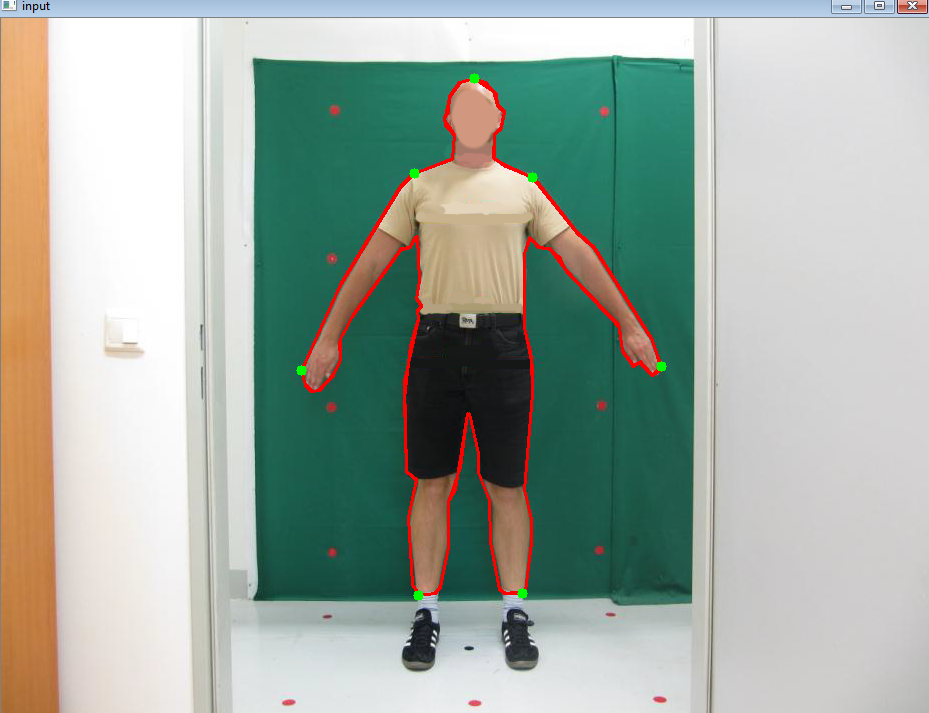
\includegraphics[width=0.5\textwidth]{body}
    \caption{Sistema de seguimiento corporal para dibujar el contorno de la persona en la
    imagen}
    \label{fig:body}
\end{figure}

Esta definición nos permite definir el proceso de inferencia como $Pr(w|x)$, es decir, la
probabilidad de que cierto estado del mundo $w$ dado $x$ dato visual. Se puede notar
rápidamente que a partir de esta definición solo se puede inferir sobre estados $w$
conocidos. Esto en práctica se resuelve utilizando un estimador $\hat{w}$ que resulte
suficientemente cercano.

\begin{figure}[H]
    \centering
    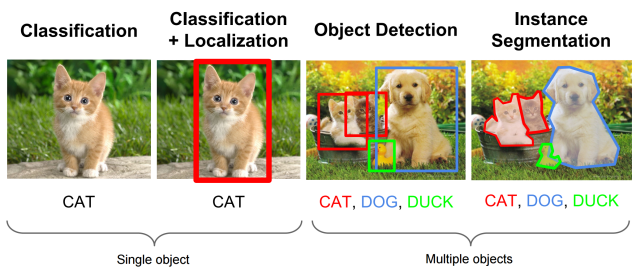
\includegraphics[width=0.8\textwidth]{obclass}
    \caption{Tipos de clasificadores de objetos; clasificación, clasificación +
    localización, detección de objetos y segmentación intensa}
    \label{fig:obclass}
\end{figure}

Para resolver un problema de visión de esta naturaleza se necesitan tres componentes:
\begin{itemize}
    \item Un modelo matemático que represente los datos visuales $x$ y los estados del
        mundo $w$. El modelo representa una familia de posibles relaciones entre $x$, 
        $w$ y la relación particular es determinada por el modelo de parámetros $\theta$.
    \item Un algoritmo de aprendizaje que nos permita ajustar los parámetros $\theta$
        usando ejemplos de pares de entrenamiento $\{x_i, w_i\}$, donde sabemos ambas
        medidas y el estado relacionado.
    \item Un algoritmo de inferencia que tome una nueva observación $x$ y use el modelo
        para calcular $Pr(w|x, \theta)$ sobre el estado del mundo $w$.
\end{itemize}

Los modelos que relacionan los datos $x$ a el mundo $w$ caen en una de dos categorías:
\begin{enumerate}
    \item modelar la contingencia del estado del mundo en los datos $Pr(w|x)$ o
    \item modelas la contingencia de los datos sobre el estado del mundo $Pr(x|w)$.
\end{enumerate}

El primer tipo de modelos es denominado discriminativo. El segundo es denominado
generativo; aquí, construimos un modelo de probabilidad sobre los datos y esto puede ser
usado para generar nuevas observaciones.

Para efectos de este informe se estudiara el primer tipo de modelo.

\subsection{Modelos de Clasificación}
Al modelar $Pr(w|x)$, elegimos un forma de distribución apropiada para $Pr(w)$ sobre los
estados del mundo $w$ y hacer la distribución de los parámetros una función de los datos
$x$. Si el mundo de estados es continuo, lo definimos como una distribución normal con
media $\mu$ en función de $x$ \cite{MLClass}.

El valor que nos entrega la función también en un conjunto de parámetros definidos,
$\theta$. Dado que la distribución dependen tanto de los datos $x$ y los parámetros
$\theta$, escribimos que la función es $Pr(w|x, \theta)$ y nos referimos a ella como
distribución posterior.

El objetivo del algoritmo de aprendizaje es el de ajustar los parámetros $\theta$ usando
pares de entrenamiento $\{x_i, w_i\}$.

\subsection{Ajuste del Modelo Probabilístico}
Nos referimos como aprendizaje al proceso de ajustar el modelo probabilístico al conjunto
de datos $\{x_i\}$ ajustando los parámetros $\theta$ y es de vital importancia que el
modelo pueda calcular la probabilidad de un nuevo dato $x*$\cite{Probab}.

\subsubsection{Regresión Logística}
Para los modelos de clasificación consideraremos la regresión logística \cite{LogicR}, la cual
independientemente de su nombre es un modelo que puede ser aplicado a clasificación. La
regresión logística es un modelo  discriminativo; nosotros seleccionamos una distribución
de probabilidad sobre un estado del mundo $w \in \{0, 1\}$ y hacemos estos parámetros
consistentes en los datos observados $x$. Como los estados del mundo son binarios,
lo describimos con una distribución de Bernoulli y hacemos el parámetro $\lambda$ (que
indica la probabilidad de que el estado del mundo tome el valor $w=1$) una medida en
función de $x$.

Es importante destacar, no podemos simplemente hacer el parámetro $\lambda$ una función
linear $\phi_0+\phi^Tx$ de las medidas; una función linear puede retornar cualquier
valor, pero el parámetro $\lambda$ debe caer entre 0 y 1. Consecuentemente, primero
debemos calcular la función linear y luego pasarla a través de la función sigmoidea que
evalúa el rango $[-\infty,\infty]$ a $[0, 1]$. El modelo final queda \ref{fig:logistic}
$$Pr(\omega|\phi_0, \phi, x)=Bern_\omega [sig[\alpha]],$$
donde $\alpha$ es denominado la activación y es dado por la función linear
$$\alpha=\phi_0+\phi^Tx$$
y donde la función sigmoidea \cite{Sigmoid} es de la forma \ref{fig:sigmoid}
$$sig(x)=\frac{1}{1 + e^{-x}}$$

\begin{figure}[H]
    \centering
    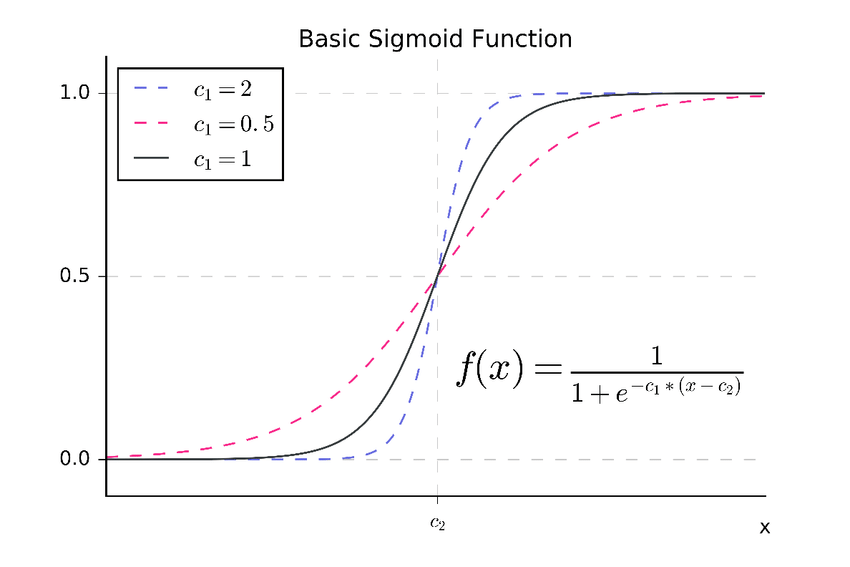
\includegraphics[width=0.6\textwidth]{sigmoid}
    \caption{Gráfica de función sigmoidea donde los valores de $c_i$ controlan la pendiente
    de la función en $c_2$}
    \label{fig:sigmoid}
\end{figure}

Así como la activación $\alpha$ tiene a infinito esta función tiende a uno. Y así como
tiende a menos infinito tiende a cero. Cuando $\alpha$ es cero, la función logística
sigmoidea retorna un valor de un medio. Para datos unidimensionales de $x$, el conjunto
de efectos de esta transformación es la de describir una curva sigmoidea relacionando $x$
con $\lambda$. La posición horizontal de la sigmoidea es determinada por el lugar donde
la función linear $\alpha$ cruza cero y su pendiente depende del gradiente $\phi_1$.

\begin{figure}[H]
    \centering
    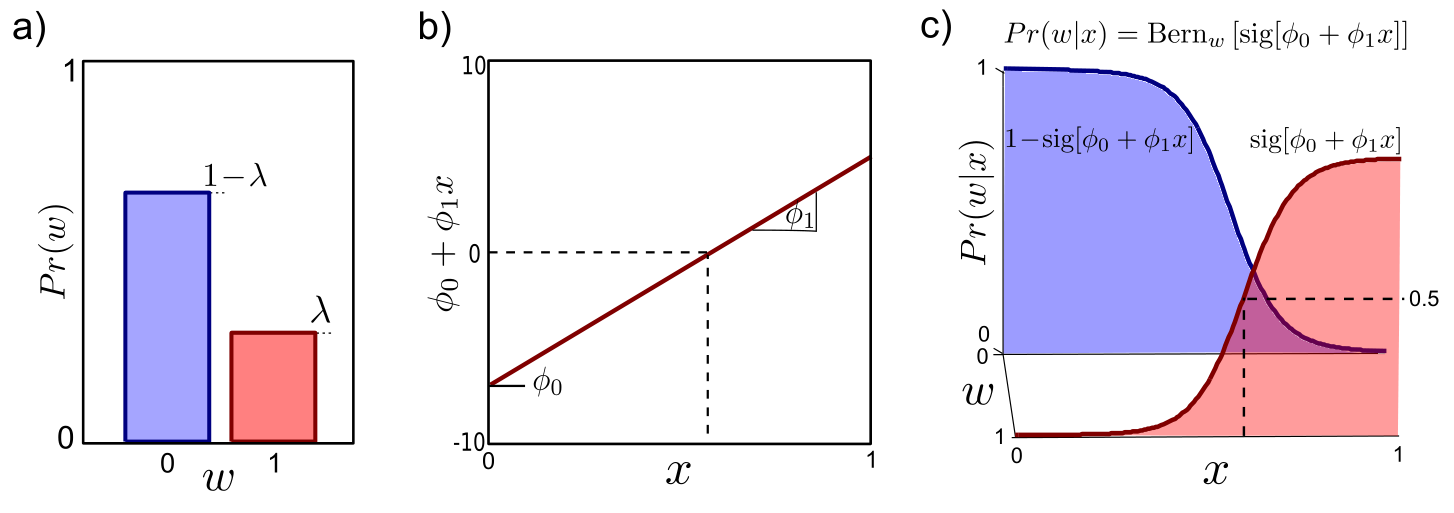
\includegraphics[width=0.8\textwidth]{logistic}
    \caption{a) representación de la probabilidad de un estado del mundo $w$ y su
        conjugado, b) función lineal de la distribución y c) función sigmoidea sobre la
        función lineal representando como los factores de la suma ponderada se anulan en torno a
    punto de diferenciación haciendo que la función defina áreas donde trabajan}
    \label{fig:logistic}
\end{figure}

\subsubsection{Método Bayesiano}
En el método bayesiano \cite{Bayes, Bayes2} dejamos de intentar estimar un solo valor de los parámetros
$\theta$ y aceptamos lo obvio; habrán muchos valores de parámetros que serán
compatibles con los datos. Calculamos la distribución de probabilidad
$Pr(\theta|x_{1...I})$ sobre los parámetros $\theta$ basados en los datos
$\{x_i\}_{i=1}^I$ usando el teorema de Bayes
$$Pr(\theta|x_{1...I})=\frac{\Pi_{i=1}^I
Pr(x_i|\theta)Pr(\theta)}{Pr(x_{1...I})}$$

Evaluando la distribución predictiva es más difícil para el caso bayesiano dado que no
tenemos ningún modelo estimado pero en su lugar encontramos una distribución de
probabilidad sobre posibles modelos. Así, calculamos
$$Pr(x*|x_{1...I})=\int Pr(x*|\theta) Pr(\theta|x_{1...I})d\theta,$$
esto puede ser interpretado como: el termino $Pr(x*|\theta)$ es la predicción para un
valor dado de $\theta$. Así, la integral puede entenderse como la suma ponderada de los
diferentes parámetros $\theta$, donde la ponderación está dada por la distribución de
probabilidad posterior $Pr(\theta|x_{1...I})$ sobre los parámetros (asumiendo que
los parámetros son diferentes).

Los cálculos de densidad predictiva para el bayesiano, máximo a posteriori u máxima
verosimilitud puede unificarse si consideramos que estos dos últimos son distribuciones
de probabilidades especiales sobre los parámetros donde toda la densidad está en
$\hat\theta$. Más formalmente, los consideramos funciones delta centradas en
$\hat\theta$. Una función delta $\delta(z)$ es una función que integra a uno, y retorna
cero en todo su dominio excepto $z=0$.

Entonces escribimos
$$Pr(x*|x_{1...I})=\int Pr(x*|\theta) \delta[\theta - \hat\theta]d\theta,$$
$$=Pr(x*|\theta),$$ 

Finalmente vemos calculamos las probabilidades evaluando la probabilidad de los datos
bajo el modelo con el que estimamos los parámetros \ref{fig:bayes}.

\begin{figure}[H]
    \centering
    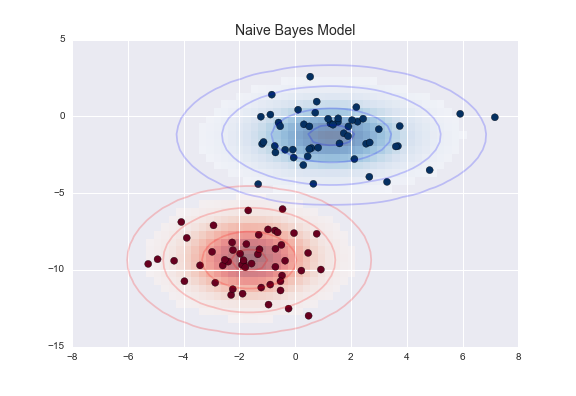
\includegraphics[width=0.8\textwidth]{bayes}
    \caption{Gráfico de funciones de datos repartidos en dos estados del mundo $w$, y el
    área de la función $Pr(x*|\theta)$ para dos estimadores (círculos en rojo y azul).}
    \label{fig:bayes}
\end{figure}

\subsubsection{Árboles de Decisión}
Para implementar ese modelo \cite{Trees} comenzamos particionando es espacio de datos en
distintas regiones y aplicamos diferentes clasificaciones a cada región.

El modelo de regresión ramificada logística tiene activaciones,
$$\alpha_i=(1-g[x_i,\omega])\phi_0^T x_i+g[x_i,\omega]\phi_1^T x_i$$

El término $g[x,\omega]$ es una función de activación que retorna un número entre 0 y 1.
Si esta función de activación retorna 0, entonces la activación será $\phi_0x_i$, por
otro lado si retorna 1, la activación será $\phi_1x_i$. Si la activación retorna un valor
intermedio, entonces la activación será la suma ponderada de los dos componentes. La
propia función de activación depende de los datos $x_i$ y toma parámetros $\omega$. Este
modelo induce un complejo límite de decisión no linear donde las dos funciones lineares
$\phi_0x_i$ y $\phi_1x_i$ son especializadas en diferentes regiones del espacio de datos.

La función de activación puede tomar muchas formas, pero una obvia posibilidad es la de
usar un segundo modelo de regresión linear. Vale decir, calculamos una función linear
$\omega^Tx_i$ de los datos que son pasados a través de una sigmoidea logística, es decir,
$$g[x_i,\omega]=sig[\omega^Tx_i]$$

Para que este modelo aprenda debemos maximizar $L = \Sigma_i \log[Pr(w_i|x_i)]$ una
probabilidad logarítmica de los pares de datos de entrenamiento $\{x_i,w_i\}_{i=1}^I$ con
respecto a todos los parámetros $\theta=\{\phi_0,\phi_1,w\}$. Normalmente esto puede
lograr usando métodos de optimización no linear.

Podemos extender esta idea para crear una estructura de árbol jerárquica anidando
funciones de activación. Por ejemplo,

\begin{equation}
    \begin{split}
        \alpha_i = (1-g[x_i, w]) \left[\phi_0^Tx_i+(1 - g[x_i,
        w_0])\phi_{00}^Tx_i+g[x_i,w_0]\phi_{01}^Tx_i\right] \\
        + g[x_i,w]\left[\phi_1^T + (1 -
        g[x_i, w_1])\phi_{01}^Tx_i + g[x_i, w_1]\phi_{11}^Tx_i\right]
    \end{split}
\end{equation}


Esto es un ejemplo de árbol de clasificación \ref{fig:tree}.

Para aprender los parámetros $\theta = \{\phi_0, \phi_1, \phi_{00}, \phi_{01}, \phi_{10},
\phi_{11}, w, w_0, w_1\}$ podemos tomar una aproximación incremental. En la primera etapa
ajustamos la parte superior del árbol, ajustando los parámetros $w, \phi_0, \phi_1$.
Luego ajustamos la rama de la izquierda, ajustando los parámetros $w_0, \phi_{00},
\phi_{01}$ y así con la rama de la derecha, ajustando $w_1, \phi_{01}, \phi_{11}$ y así
sucesivamente.

\begin{figure}[H]
    \centering
    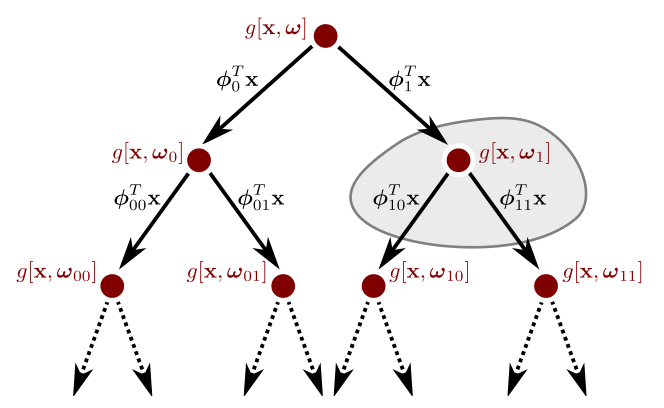
\includegraphics[width=0.7\textwidth]{tree}
    \caption{Árbol de clasificación definido para el ejemplo donde los datos fluyen desde
        la raíz hasta las hojas. El área en gris representa el área de las variables que
    pueden ser desarrolladas juntas en un entrenamiento incremental.}
    \label{fig:tree}
\end{figure}

\subsubsection{Bosque de Árboles Aleatorio}
Esta idea se volvió popular en la problemas de clasificación multiclase usando la idea
de árbol de decisión definida anteriormente.

Un bosque aleatorio \cite{Forest} es una colección de árboles aleatorios, cada uno de
estos usa un conjunto de funciones elegidas de manera aleatoria. Cuando se promedian
todas las probabilidades de cada árbol, es decir, $Pr(x*|w_i)$ predicha por cada árbol, se
produce una clasificación mucho más robusta. Una forma de pensarlo es aproximarlo al
método bayesiano; donde construimos una respuesta final tomando una suma ponderada de las
predicciones propuestas por los distintos conjuntos de parámetros \ref{fig:forest}.

\begin{figure}[H]
    \centering
    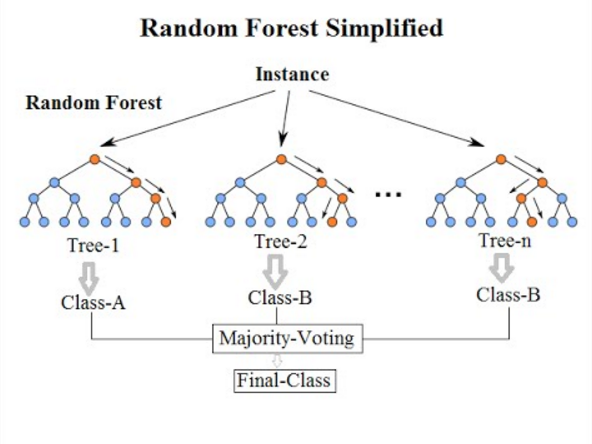
\includegraphics[width=0.8\textwidth]{forest}
    \caption{N instancias de árboles generando inferencia sobre un dato $x$ y ponderando
    su resultado en una votación para generar la predicción final.}
    \label{fig:forest}
\end{figure}

% Metodología de cs (Data augmentation, Data cleaning, Balancing)
\subsection{Conjunto de Datos}
El manejo de los conjuntos de datos \cite{Manage} es una de las tareas más importantes a la hora de
diseñar un modelo de IA, ya que la información y como esté clasificada marcará como el
modelo podrá desempeñarse en un entorno de uso general o específico que no contenga
información vista con anterioridad.

La estructura general de un conjunto de datos en modelos de visión por computadora suele
consistir en un conjunto de imágenes o videos junto a etiquetas que muestran la
información contenida en estas, normalmente en la forma de coordenadas que delimitan el
área en donde se localiza en la imagen el objeto a identificar y/o clasificar, junto a la
etiqueta que identifica que es o que acción esta ocurriendo.

Es importante contar con un conjunto de datos que contenga gran cantidad de ejemplos
relacionados a la tarea que se espera lograr, esto con objetivo de generalizar los
patrones e información obtenida por parte del modelo durante el proceso de entrenamiento.
La cantidad de información que se requiera estará dada por la complejidad en el modelo a
entrenar y la complejidad de la tarea a desarrollar, y el análisis de estos parámetros
dependerá del equipo de desarrollo. Cuando en entrenamiento carece de un conjunto de
datos contundente o el modelo es muy simple para la tarea ocurre \textit{underfiting},
esto es, cuando el modelo realiza inferencias escazas y/o erróneas.

Para un hacer buen provecho de la información existen diferentes tratamientos realizables
a los conjuntos de datos como lo son el limpieza de datos, aumento de datos y el balanceo
de datos.

\subsubsection{Limpieza de Datos}
La limpieza de datos es un procedimiento que nos ayuda a filtrar datos erróneos y
manipular información faltante para no causar una mayor perdida de datos \cite{Clean}.
Este procedimiento es descrito como la intuición de los datos, dado que no existen muchas
más formas de entender un conjunto de datos que analizándolo de manera manual.
Generalmente el manejo de la limpieza de datos suele ser una de las partes más
demandantes en el proceso de desarrollo de un modelo de inteligencia artificial.

Los problemas que se presentan en conjuntos de datos que debes ser solventados son:
\begin{itemize}
    \item \textbf{Datos faltantes}: Existen situaciones en las que no todos los datos de una
        entrada tendrán asignados un valor. Si bien es factible eliminar todas las
        entradas que contengan datos perdidos, en la mayoría de los casos esto termina
        descartando excesiva cantidades de entradas (hay conjuntos de datos que pueden
        tener datos perdidos en todas sus entradas).

        Una alternativa para cuando los datos faltantes tienen estar agrupados en su
        mayoría en un campo en particular es eliminar el campo por completo. Esto valido
        dado que el campo de por si mostraba no tener mucha utilidad.

        La forma más común de manejar datos faltantes es usar un valor por defecto que en
        ultima instancia servirá para que el modelo reconozca que existen situaciones
        donde los datos no se encuentran disponibles. Esto es básicamente porque siempre
        se puede extraer información del echo de que no existen entradas en un campo en
        particular \cite{Miss}.
    \item \textbf{Distribución de datos inconsistentes}: Esto ocurre cuando la escala o
        el formato de los datos no esta bien definido en los campos, vale decir, tener
        números en campos que describen texto o números en rangos que no corresponden.

        Cuando se habla de inconsistencia en tipo de datos solo basta con reconocer el
        tipo de dato del campo para hacer la corrección del resto de los datos, revisando
        que la transformación de los datos sea consistente al objetivo final.

        Cuando la inconsistencia corresponde a rangos se implementan dos alternativas,
        escalado y normalización.

        El escalado corresponde a una transformación en el rango de los datos, esto
        convierte los datos tomando el mínimo y máximo valor en los campos y escalándolos
        a valores entre 0 y 1.

        La normalización es una transformación que convierte la distribución de los datos
        en una distribución normal Gaussiana. Este método es utilizado en datos
        destinados a modelos de predicción estadística \cite{Scal}.
    \item \textbf{Datos inconsistentes}: Es el tipo de dato que requiere manipulación
        acorde a las necesidades, estos datos pueden ser desde texto que registra
        entradas diferentes por tener su versión iniciando con mayúsculas y su versión en
        minúsculas hasta tipos de datos diferentes en las mismas columnas.

        Para la reparación de estos datos se debe hacer estudio de los datos y la
        información que se espera de ellos y es totalmente sujeta a quien manipula los
        datos \cite{Ingsoc}.
\end{itemize}
\subsubsection{Aumento de Datos}
Muchos de los desarrollos de modelos actuales presentan una característica en común,
fueron entrenados con cantidades de datos que pasan el orden de magnitud de los cientos
milos o millones. Esto es un importante dato a considerar cuando se tienen modelos que
no cuentan con un conjunto de datos lo suficientemente amplio \ref{fig:dataaugmen}
\cite{Dataaug}.

\begin{figure}[H]
    \centering
    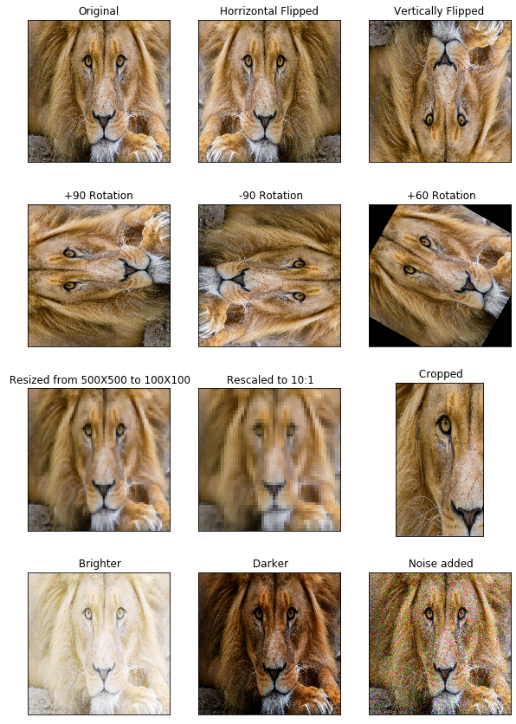
\includegraphics[width=0.8\textwidth]{dataaugmen}
    \caption{Ejemplo de aumento de datos, las transformaciones incluyen la imagen
        original, reflejo horizontal, reflejo vertical, rotaciones de 90°, -90° y 60°,
        reescalado a una menores resoluciones, recortes, aumento y disminución de exposición y
    agregación de ruido aleatorio.}
    \label{fig:dataaugmen}
\end{figure}

Para esto es que se hacen estudios respecto el aumento artificial de datos, que consisten
en resumidas cuentas en el uso de datos pre-existentes en el conjunto de datos actual
para creas nuevas entradas que representen información similar. Hay estudios que muestran
aumentos de rendimiento sobre el 30\% \cite{Augment} sobre modelos que no la utiliza.

\subsubsection{Aumento de datos numéricos}
Las técnicas de aumento utilizadas \cite{Augment2} en las aplicaciones de aprendizaje
profundo dependen del tipo de datos. Para aumentar los datos numéricos simples, son
populares técnicas como \textit{SMOTE, ADASYN o RandomOverSampler}\ref{fig:smote}. Estas
técnicas se utilizan generalmente para abordar el problema del desequilibrio de clases en
las tareas de clasificación. 

\begin{figure}[H]
    \centering
    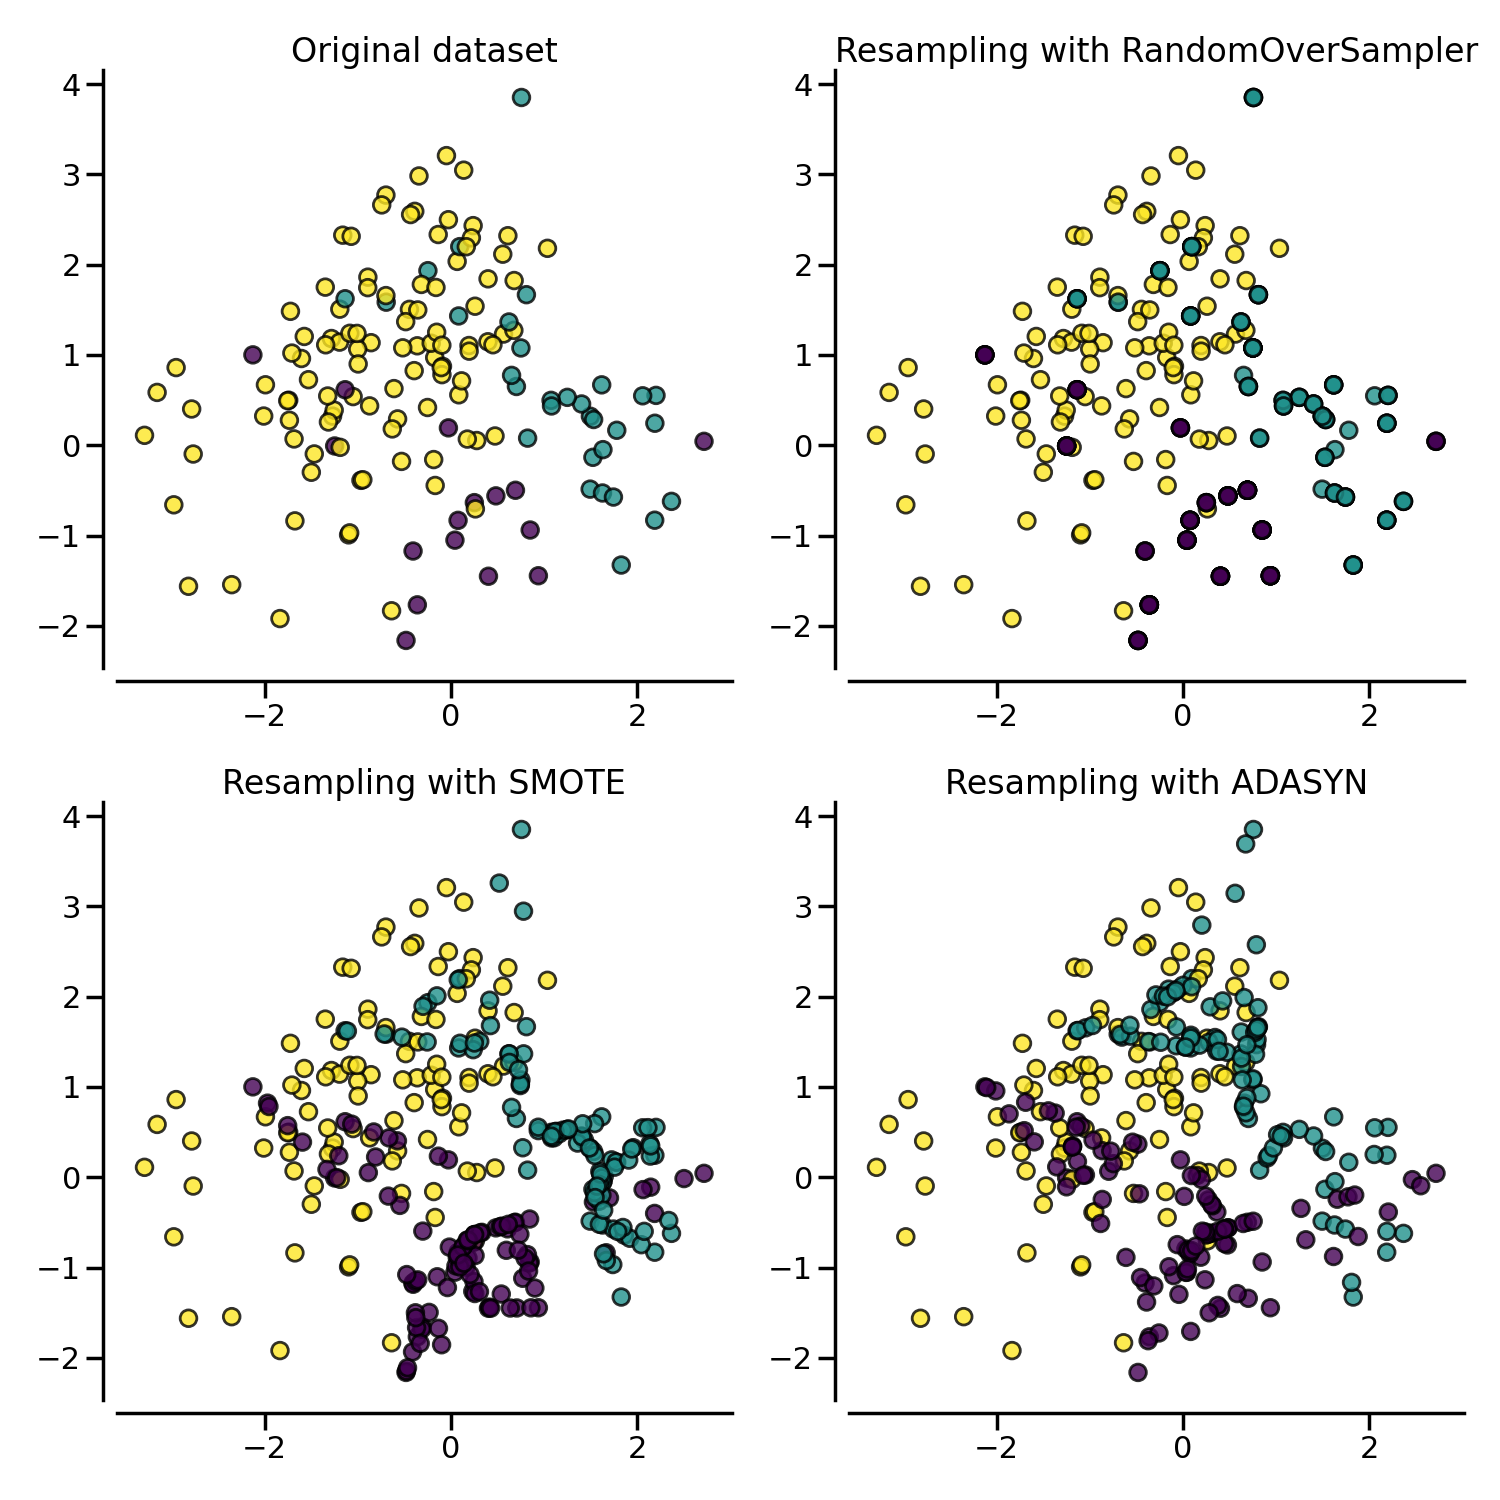
\includegraphics[width=0.8\textwidth]{smote}
    \caption{\textit{Original dataset} muestra el conjunto de datos original,
        \textit{RandomOverSampler} muestra el aumento de datos de manera aleatoria,
        \textit{SMOTE} muestra el aumento de datos más localizado y \textit{ADASYN} muestra el
    aumento de muestras para definir zonas más marcadas.}
    \label{fig:smote}
\end{figure}

Para los datos no estructurados, como las imágenes y el texto, las técnicas de aumento
varían desde simples transformaciones hasta datos generados por redes neuronales, en
función de la complejidad de la aplicación \cite{Augment3}.

\subsubsection{Balanceo de Datos}
En cierto tipo de conjuntos de datos ocurre que cierta concentración de datos sobrepasa
de sobre manera a otra, causando desbalanceo de datos. Una forma de sobre llevar esto es
particionando el segmento de datos más abundante para poder representar toda la
información con el mismo nivel de importancia \ref{fig:balance} \cite{Balan}.

\begin{figure}[H]
    \centering
    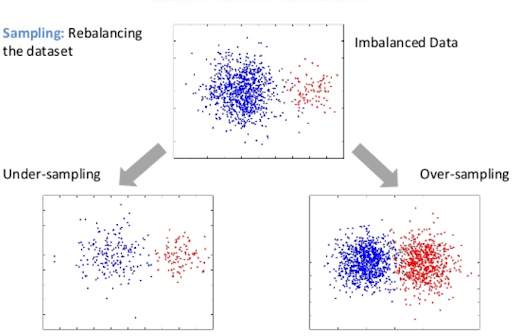
\includegraphics[width=0.8\textwidth]{balance}
    \caption{En \textit{Under-samplig} se eliminan datos del grupo más cuantioso para
        igualar proporciones, en cambio, en \textit{Over-samplig} se aumentan de manera
    artificial los datos del grupo con menos representación.}
    \label{fig:balance}
\end{figure}

Es importante reconocer las desventajas a lo que esto puede con llevar; esto hace dejar
de lado gran cantidad de datos, esto es proporcional al conjunto que represente la
minoría de datos en el conjunto, esto culminando en \textit{underfiting}.

% Modelos de cv
% Segmentación
\subsection{Segmentación}
La segmentación \cite{Segmenta} de imágenes es el tipo de modelo que delimita los
contornos de los elementos contenidos en la entrada visual, en este modelo cada pixel
pertenece a una clase. Es usado para identificar imágenes para aplicaciones que requieren
gran nivel de precisión. La salida es una máscara que delimita la forma del objeto en la
imagen. La segmentación de imágenes viene en muchas formas (segmentación semántica,
intensa, panóptica, etc.), la práctica de segmentación de imágenes generalmente describe
la necesidad de anotar cada pixel de la imagen con una clase.

\begin{itemize}
    \item \textbf{Segmentación de instancias}: cada instancia de un objeto es etiquetada por
        separado y los segmentos sin instancia son ignorados.
        \begin{figure}[H]
            \centering
            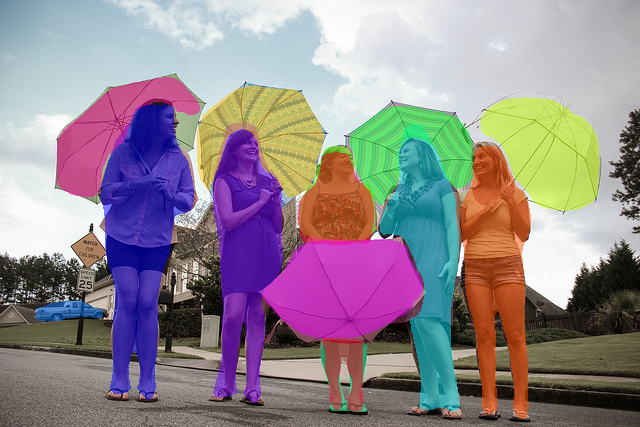
\includegraphics[width=0.6\textwidth]{segment3}
            \caption{Ejemplo de segmentación de instancias donde se puede ver que cada
                elemento reconocido recibe un color diferente. Elementos como los carteles
            o árboles del fondo al no contar con etiqueta son ignorados por el modelo.}
            \label{fig:segment3}
        \end{figure}
    \item \textbf{Segmentación semántica}: Aquí se consideran todas las regiones de la
        imagen y los objetos del mismo tipo reciben la misma etiqueta.
        \begin{figure}[H]
            \centering
            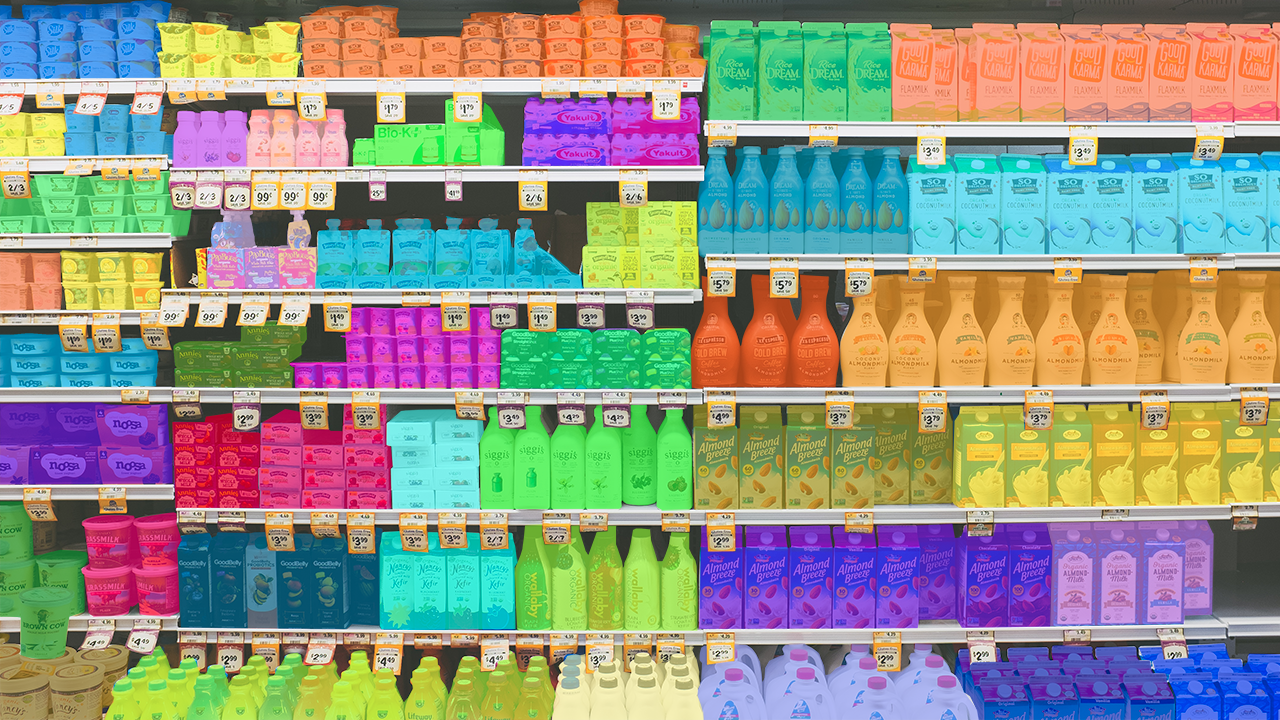
\includegraphics[width=0.6\textwidth]{segment2}
            \caption{Ejemplo de segmentación semántica donde los objetos similares son
            agrupados bajo la misma etiqueta}
            \label{fig:segment2}
        \end{figure}
    \item \textbf{Segmentación panóptica}: es una combinación de segmentación semántica y
        segmentación de instancias, de modo que a todos los píxeles se les asigna una
        etiqueta de clase y todas las instancias de objetos están segmentadas de forma
        única.
        \begin{figure}[H]
            \centering
            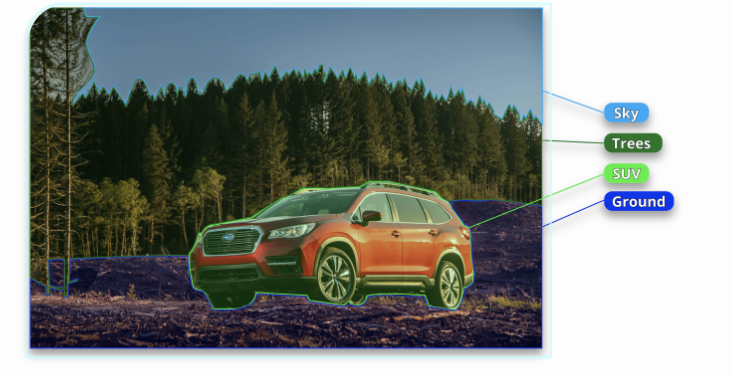
\includegraphics[width=0.7\textwidth]{segment}
            \caption{Ejemplo de segmentación panóptica donde la totalidad de la imagen
                recibe una clase que diferencia los distintos objetos contenidas en esta. En
                la parte superior el cielo, los árboles de fondo, el vehículo en primer plano el
            suelo debajo de este.}
            \label{fig:segment}
        \end{figure} 
\end{itemize}

% Tipo de imágenes (microscópicas)
\subsection{Procesamiento de Imágenes y Extracción de Características}
Es importante saber reducir la complejidad del análisis de imágenes sabiendo reconocer
que tipo de solución necesitamos para nuestro problema. Para ello existen multiples
transformaciones que permiten simplificar la entrada visual que recibirá el modelo en
orden de facilitar la tarea de extracción de características claves \cite{Prince}.

\subsubsection{Transformación por Pixel}
Es la transformación más directa de imágenes \cite{Pixel}, consisten en la modificación de
pixeles individuales asumiendo la estructura bidimensional. Se dice que la transformación
modifica el pixel $p_{ij}$ donde $i, j$ son las coordenadas del pixel en el arreglo de la
imagen $P$.

\subsubsection{Escala de Grises}
Es convertir la imagen de entrada a color a su versión a escala de grises. Este filtro es
especialmente útil para reducir el arreglo de pixeles de valores rgb a un simple valor
que representa el nivel de blanco del pixel, esto es útil en los casos donde los colores
no son relevantes en la extracción de características \cite{Pixel}.

\begin{figure}[H]
    \begin{subfigure}{0.5\textwidth}
        \centering
        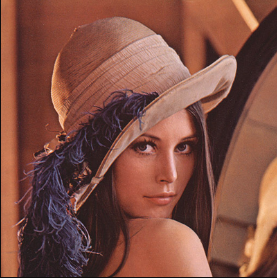
\includegraphics[width=0.8\textwidth]{color}
        \caption{Versión de imagen a color.}
        \label{fig:color}
    \end{subfigure}
    \begin{subfigure}{0.5\textwidth}
        \centering
        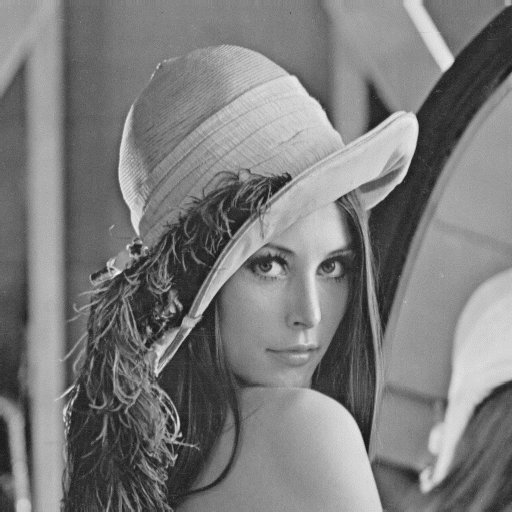
\includegraphics[width=0.8\textwidth]{gray}
        \caption{Versión de imagen en escala de grises.}
        \label{fig:gray}
    \end{subfigure}
    \caption{Transformación de imagen en su escala de grises.}
    \label{fig:lenna}
\end{figure}

\subsubsection{Filtros Lineales}
Son transformaciones de pixeles $x_{ij}$ que consideran una suma ponderada del valor de
los pixeles adyacentes \cite{Conv}, es decir, siendo una imagen $P$ a la cual se  aplicará
un filtro denominado \textit{kernel} $F$, el cual tendrá entradas $f_{mn}$ donde
$m\in\{-M,M\}$ y $n\in\{-N,N\}$. Finalmente quedamos con un filtro de la forma
\ref{fig:kernel}
$$x_{ij}=\Sigma_{m=-M}^M\Sigma_{n=-N}^Np_{i-m,j-n}f_{m,n}$$

\begin{figure}[H]
    \centering
    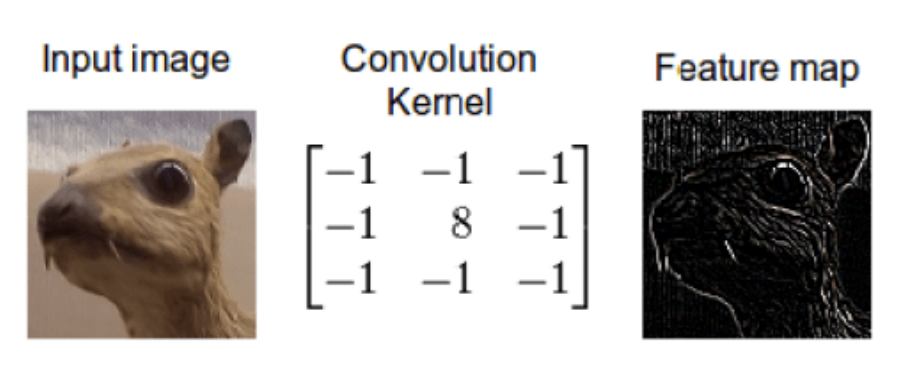
\includegraphics[width=0.8\textwidth]{kernel}
    \caption{Filtro con \textit{kernel} para resaltar contornos de objetos en la imagen.
        La matriz se usa para saber las ponderaciones de los pixeles en la suma para el nuevo
        valor de pixeles en la imagen. Así obtenemos un mapa de características que en este
    ejemplo nos entrega la información de los límites del animal de la imagen de entrada.}
    \label{fig:kernel}
\end{figure}

%\section{Estado del Arte}\label{arte}
% Alternativas preexistentes
% Conjuntos de datos preexistentes

\chapter{Formulación del Proyecto}\label{formulación}

\section{Objetivo General}
Crear un modelo de aprendizaje de maquinas para la detección de y clasificación de
parásitos en el análisis parasitológico de seriado de deposiciones.

\section{Objetivos Específicos}
\begin{enumerate}\justifying
    \item Recopilar y estructurar un conjunto de datos de imágenes de muestras para el entrenamiento y testeo del modelo de detección de parásitos.
    \item Definir un modelo de detección de parásitos para la automatización de resultados del examen parasitológico seriado de deposiciones basado en visión por computadora.
    \item Analizar y validar la calidad de las predicciones de la detección de parásitos en
        las muestras, a través de experimentación con el conjuntos de datos recopilado y
        con muestras obtenidas desde procedimientos reales del examen parasitológico
        seriado de deposiciones, utilizando imágenes microscópicas.
\end{enumerate}

%\section{Justificación}
%Que se planea realizar y hasta que punto se espera llegar.
%
%Esta subdivisión debe:
%\begin{enumerate}\justifying
%\item Identifique el producto del software para ser diseñado por el nombre (por ejemplo, Anfitrión DBMS, el Generador del Reporte, etc.);
%\item Explique eso que el producto (del software hará y que no hará.
%\item Describe la aplicación del software especificándose los beneficios pertinentes, objetivos, y metas;
%\item Sea consistente con las declaraciones similares en las especificaciones de niveles superiores (por ejemplo, las especificaciones de los requisitos del sistema), si ellos existen.
%\end{enumerate}
%\blindtext

\section{Metodología}
\begin{enumerate}\justifying
    \item Recopilar y estructurar un conjunto de datos de imágenes de muestras para el entrenamiento y testeo del modelo de detección de parásitos.
        \begin{enumerate}
            \item Formulación del proyecto.
            \item Revisión de la literatura relacionada al proyecto de título.
            \item Desarrollo del marco teórico.
            \item Escritura del informe.
            \item Revisión de conjunto de datos disponibles relacionados al examen
                parasitológico seriado de deposiciones.
            \item Definir una estructura estándar para almacenar imágenes microscópicas
                de examen parasitológico seriado deposiciones.
            \item Implementar un procedimiento de extracción y limpieza de imágenes de
                examen parasitológico seriado de deposiciones.
            \item Realizar un procedimiento de análisis exploratorio de datos.
        \end{enumerate}

    \item Definir un modelo de detección de parásitos para la automatización de resultados del examen parasitológico seriado de deposiciones basado en visión por computadora.
        \begin{enumerate}
            \item Adoptar una metodología (elección de experimento, métricas, configuración
                y \textit{kfolds}) de proyectos de visión por computadora para realizar una
                comparación de la calidad de los modelos.
            \item Proponer distintos modelos para la detección de parásitos en imágenes
                microscópicas.
            \item Seleccionar el o los modelos con mejor calidad de resultado.
        \end{enumerate}

    \item Analizar y validar la calidad de las predicciones de la detección de parásitos en
        las muestras, a través de experimentación con el conjuntos de datos recopilado y
        con muestras obtenidas desde procedimientos reales del examen parasitológico
        seriado de deposiciones, utilizando imágenes microscópicas.
        \begin{enumerate}
            \item Implementar la metodología elegida o adaptada para el tratamiento de
                imágenes microscópicas.
            \item Implementar el procedimiento de predicción de parásitos detectada en las
                imagen microscópicas.
            \item Implementar el reporte final de parásitos detectados en las muestras a
                través del modelo de visión por computadora.
            \item Recopilación de nuevas muestras, sus resultados, su validación y la
                retroalimentación del tecnólogo médico.
        \end{enumerate}
\end{enumerate}

%\subsubsection{Equipo de Trabajo}
%Content ;v
% Calza esto
% 1
% 2-3.5
% 3-4

\subsection{Planificación}
\begin{figure}[H]
    \centering
    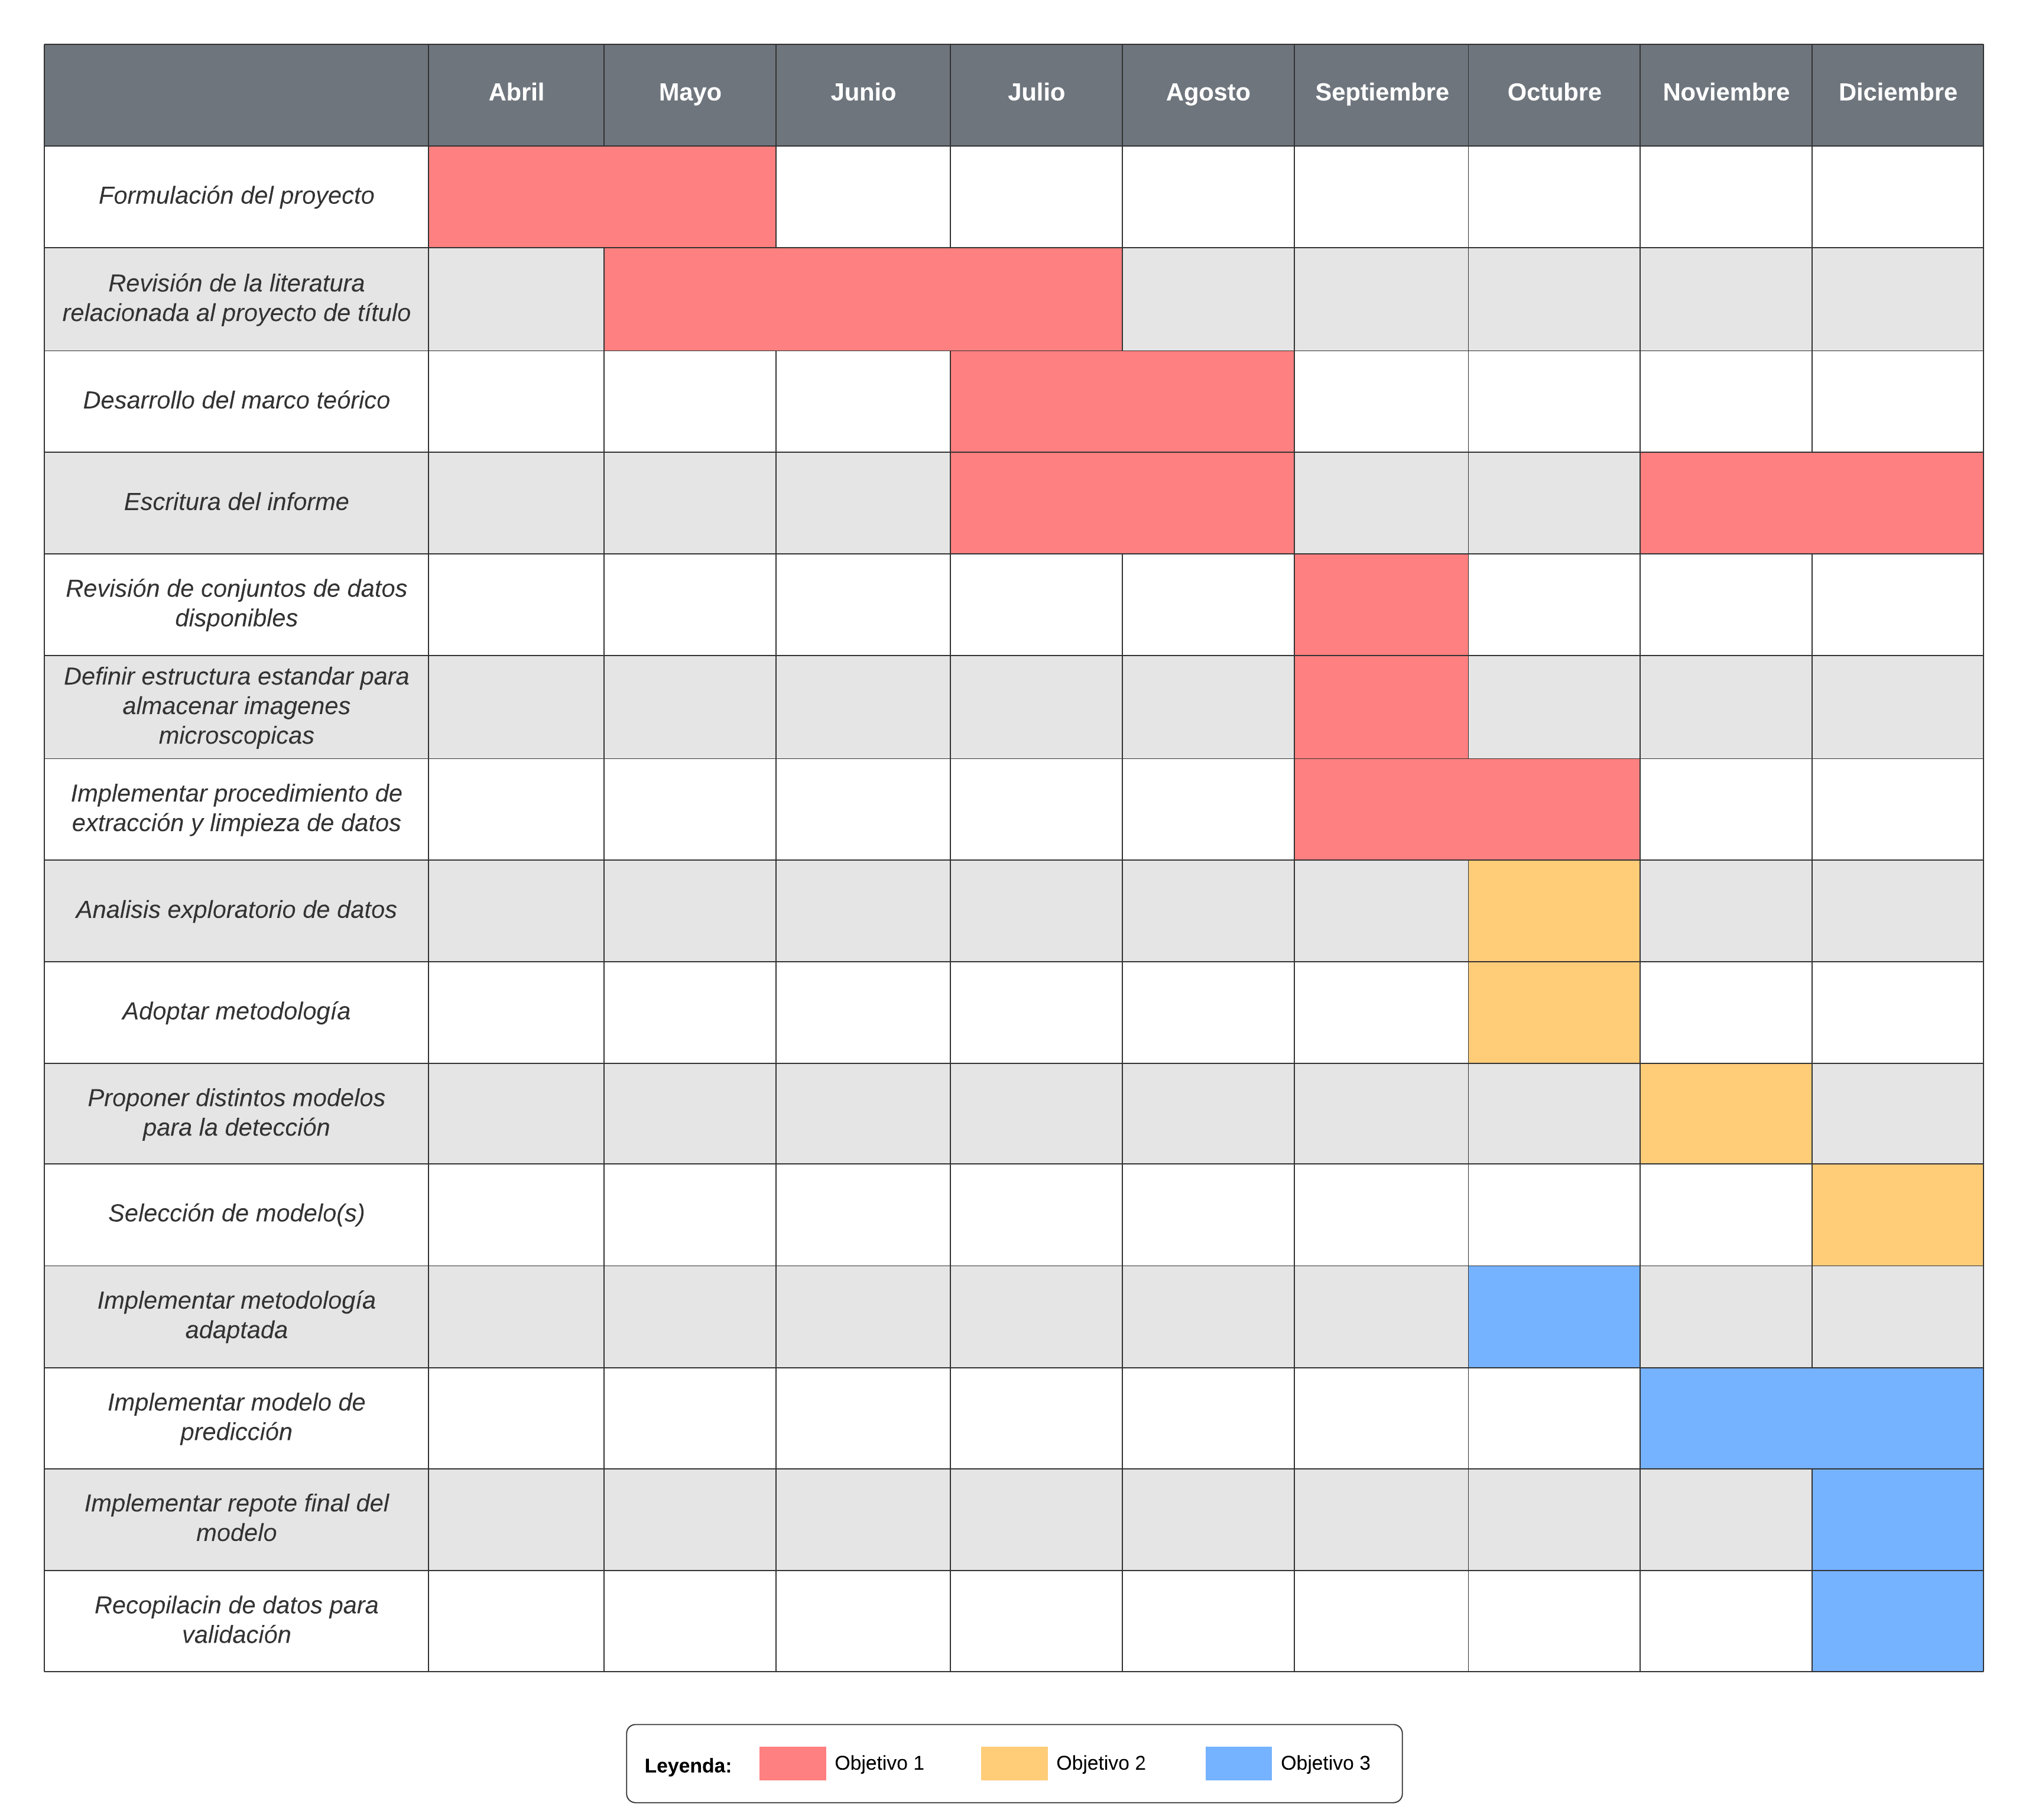
\includegraphics[width=0.9\textwidth]{gantt}
    \caption{Carta Gantt para desarrollo del proyecto}
    \label{fig:gantt}
\end{figure}

\section{Desarrollo}
\subsection{Conjunto de Datos}
Para el desarrollo del proyecto de título se utiliza el conjunto de datos \textit{Makerere
Automated Lab Diagnostics Database (MALDD)} en cuyas característica encontramos 1217 imágenes 
clasificadas entre tres distintas clases de parásitos:

\begin{itemize}
    \item Hookworm
    \item Hymenolepsis Nana
    \item Taenia
\end{itemize}

El conjunto se compone de imágenes microscópicas de muestras de heces fecales y su
clasificación destaca cualquier presencia de los parásitos anteriormente mencionados. 
La estructura de los datos se conforma en una carpeta raíz con las imagenes y su meta data
en un archivo en formato \textit{xml}, ambos de mismo nombre.

\begin{lstlisting}[language=xml]
<annotation>
  <source>
    <database>Makerere Automated Lab Diagnostics Database</database>
    <annotation>Makerere University</annotation>
    <image>Mulago National Referral Hospital</image>
  </source>
  <size>
    <width>2064</width>
    <height>1161</height>
  </size>
</annotation>
\end{lstlisting}

\begin{figure}[ht]
    \centering
    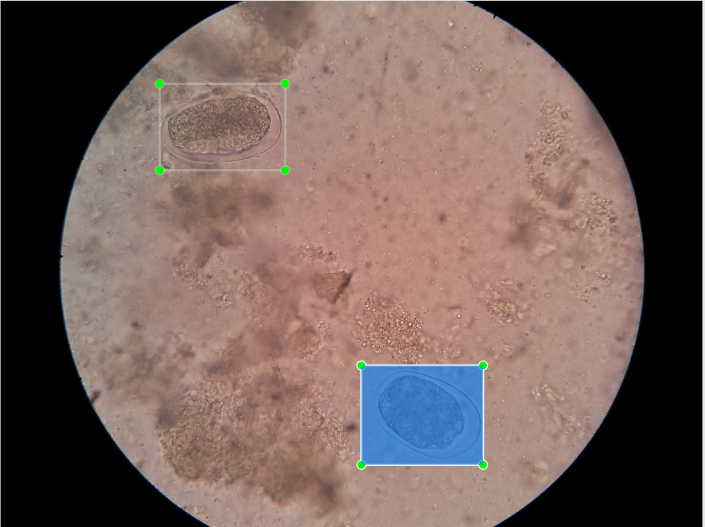
\includegraphics[width=0.8\textwidth]{labelImage}
    \caption{Ejemplo de imagen donde se aprecian dos \textit{Hookworms}.}
    \label{fig:labelImage}
\end{figure}
% TODO: poner más fotos de las otras dos clases

El proceso de preprocesamiento y limpieza de datos comprente la reestructuración de las
captetas separando el conjunto en entrenamiento (\textit{train}) y testeo (\textit{test}),
a su vez se requiere de una modificación en la meta data de los archivos \textit{xml}
que incluya si la carpeta del archivo corresponde a uno de entrenamiento o testeo, agregar
un tag con el nombre del archivo de la imagen que le corresponde y su ruta absoluta al mismo.

\begin{figure}[ht]
    \centering
    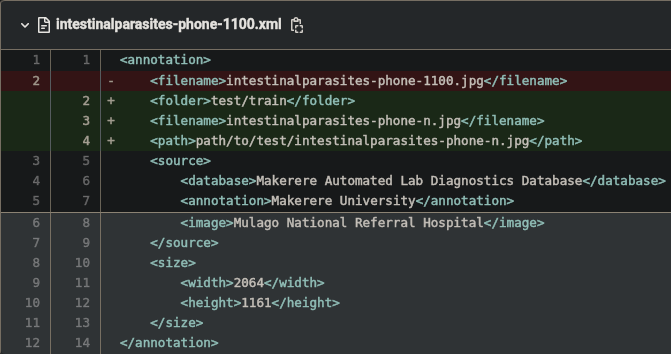
\includegraphics[width=0.9\textwidth]{diff}
    \caption{Ejemplo de modificación de archivo \textit{xml} de imagen n.}
    \label{fig:diff}
\end{figure}

La utilidad de conjunto de datos está especialmente orientada a la detección de estas clases
en el contexto descrito. En el contexto del examen parasitologico seriado de deposiciones,
el conjunto de datos cubre una pequeña parte de los parásitos que se esperan reconocer.

La expansión esperada del conjunto de datos es abarcar las clases faltantes compuestas por:

\begin{itemize}
    \item Aedes aegypti
    \item Anisaki spp
    \item Anopheles
    \item Ascaris lumbricoide
    \item Balantidium coli
    \item Blastocystis hominis
    \item Chilomastix mesnili
    \item Cryptosporidium spp
    \item Cyclospora cayetanensis
    \item Cystoisospora belli
    \item Diphyllobothrium spp
    \item Endolimax nana
    \item Entamoeba coli
    \item Entamoeba gingivalis
    \item Entamoeba histolytica / dispar
    \item Enterobius vermicularis
    \item Fasciola hepática
    \item Giardia lamblia
    \item Hymenolepis diminuta
    \item Iodamoeba butschlii
    \item Latrodectus mactans: viuda negra
    \item Loxosceles laeta: rincon
    \item Schistosoma mansoni
    \item Toxoplasma gondii
    \item Tribolium confusum
    \item Trichomonas tenax
    \item Trichomonas vaginalis
    \item Trichuris trichiuria
    \item Trypanosoma cruzi
    \item Pediculus humanus
    \item Plasmodium falciparum
    \item Phthirus pubis
    \item Pulex irritans
    \item Schistosoma haematobium
\end{itemize}

\subsection{Modelo}

% TODO: explicar Resnet y Centernet
Se revisaron las opciones de modelos; \textit{Faster RCNN Inception Resnet v2 (FRIR v2)} y
\textit{Centernet} durante la face de investigación con el objetivo de un modelo general que
pueda especificarse en la tarea de reconocimiento de parásitos a través de imágenes
microscópicas.

Se descarta \textit{FRIR v2} por su lento desempeño general en inferencias sobre conjuntos
de datos de imagenes de contexto general.

Finalmente se decide por \textit{Centernet} por su característica forma de realizar una
infernecia, \textit{Centernet} busca identificar ejes aliniados a un rectangulo
correspondiente a un objeto dentro de una imagen. Esta diferencia nace de su forma de 
buscar regiones que contengan objetos e identeficandolos como un punto, dando así con un
modelo de muy rápida inferencia y gran nivel de presición en casos particulares.

\begin{figure}[ht]
    \centering
    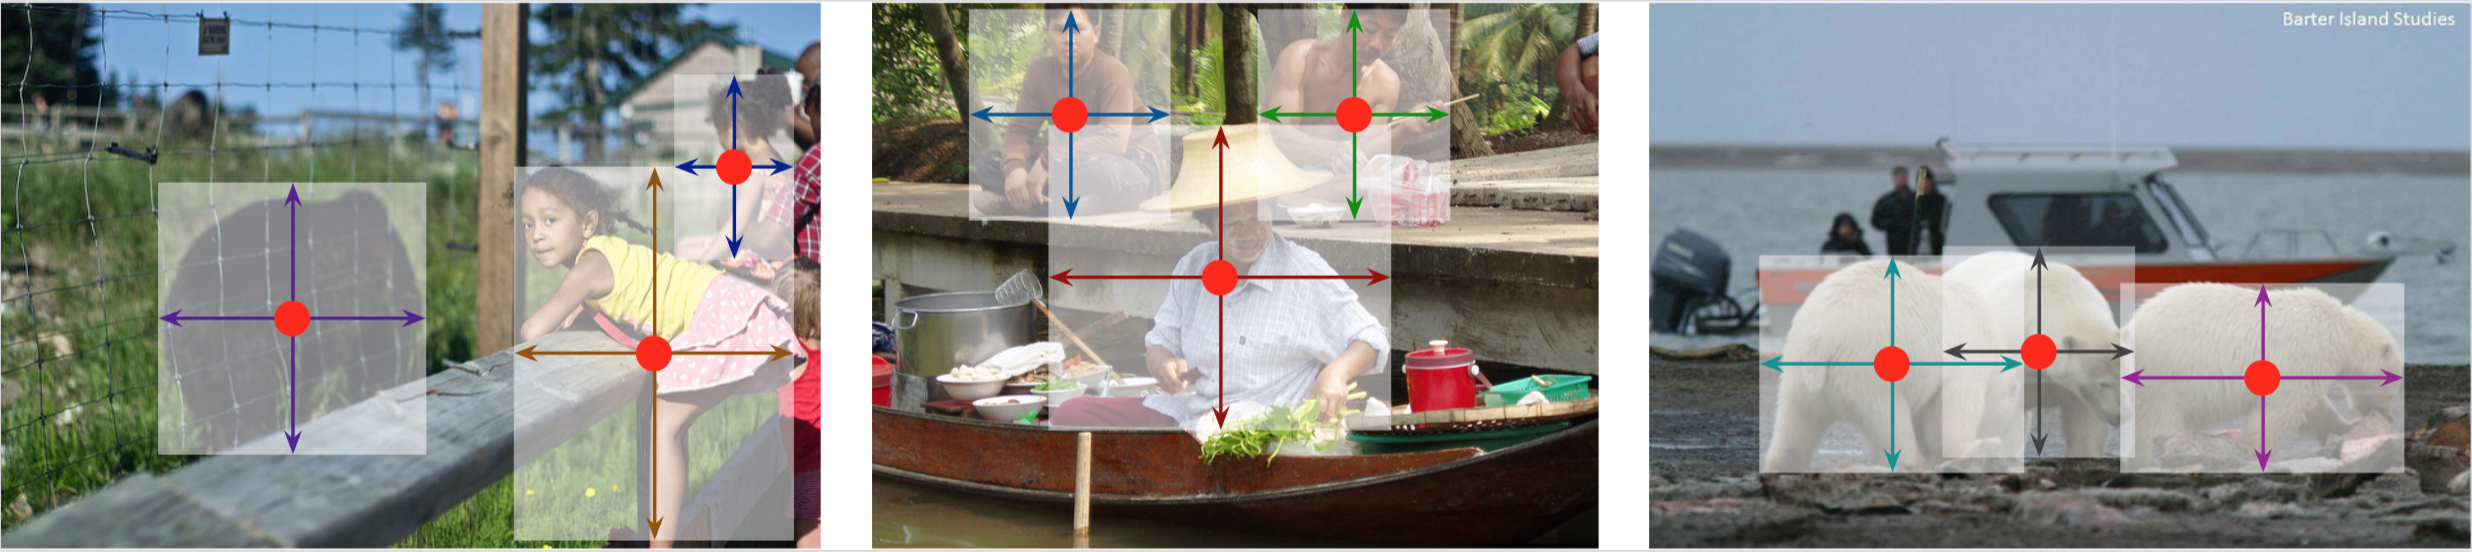
\includegraphics[width=0.8\textwidth]{centernet}
    \caption{Ejemplo de detección de objetos con \textit{Centernet}.}
    \label{fig:centernet}
\end{figure}

\subsection{Entrenamiento}
% TODO: explicar tensorflow api
El entrenamiento del modelo \textit{Centernet} con el conjunto de datos de \textit{MALDD} se
realiza de manera local con la API de \textit{TensorFlow} para un seguimiento en tiempo real
de las mediciones de pérdida del modelo durante el entrenamiento.

Especificaciones del computador usado durante la etapa de entrenamiento:

\begin{itemize}
    \item Procesador: AMD 2600X (6 núcleos)
    \item Tarjeta Gráfica: NVidia RTX 2060 (6GB)
    \item Cantidad de Memoria RAM: 16 GB
\end{itemize}

\subsection{Resultados}
% TODO: graficos de perdida
\blindtext

%\subsection{Desglose de Actividades}\label{PERT}
%En esta sección se describen cada una de las actividades, duración, dependencias, caminos críticos, entre otras y se debe dar una conclusión de lo mismo.
%\begin{figure}[hbt]
%\begin{tabular}{|c|c|c|c|c|}\hline
%\textbf{Actividad}&\textbf{Duración} &\textbf{Después de} & \textbf{Simultanea} & \textbf{Antes de}\\\hline
%& & &&\\\hline
%
%\end{tabular}
%\caption{Duración de tareas y dependencias}
%\end{figure}
%
%\begin{landscape}
%\begin{figure}[hbt]
%\centering
%%\includegraphics{}
%\caption{Grafo de Actividades del Proyecto XYZ}
%\label{CPM}
%\end{figure}
%\end{landscape}
%
%\begin{landscape}
%\begin{figure}[hbt]
%\centering
%%\includegraphics{}
%\caption{Grafo de Actividades con duración del Proyecto XYZ}
%\label{CPMduracion}
%\end{figure}
%\end{landscape}
%
%\begin{figure}[hbt]
%\begin{tabular}{|c|c|cc|cc|c|c|}\hline
%& & \multicolumn{2}{|c|}{\textbf{Inicio}} & \multicolumn{2}{|c|}{\textbf{Termino}} & \textbf{Holgura} & \\
%\textbf{Actividad}& \textbf{Duración}& \textbf{Temprano} &\textbf{Tardío} &\textbf{Temprano} &\textbf{Tardío} &\textbf{Total}  &\textbf{Crítico} \\\hline
%& & &   & &   & & \\\hline
%
%\end{tabular}
%\caption{Cálculo del diagrama de actividades}
%\end{figure}
%
%\begin{landscape}
%\begin{figure}[hbt]
%\centering
%%\includegraphics{}
%\caption{Grafo de Actividades con duración y caminos críticos}
%\label{CPMcritico}
%\end{figure}
%\end{landscape}

\chapter{Conclusión}\label{conclusion}
Durante este informe se vieron las tecnologías relacionadas a la visión por computadora
que permiten hacer uso de una inferencia en base al entrenamiento de modelos de
aprendizaje de máquinas para la detección y clasificación de presencia parasitológica en
el examen seriado de deposiciones. Vimos el estado de los procedimientos para este examen
y reconocimos el punto donde el uso de estas tecnologías puede jugar un gran rol en la
mejora de resultados y la velocidad de análisis.
%\section{Principales aportes}
%\section{Contraste de resultados}
%\section{Trabajos futuros} Solo si corresponde.

%%%%%REFERENCIAS
\renewcommand{\refname}{Referencias}

%agregar referencias
\bibliographystyle{apacite}\bibliography{document.bib}

%\renewcommand{\appendixname}{Anexos}
%\appendix
%
%\chapter{Definciones, Acronimos y Abreviaturas}\label{definiciones}
%\section{Definiciones}
%\section{Acrónimos}
%\section{Abreviaturas}
%
%\chapter{Configuraciones}\label{configuracion}
%\blindtext %reemplazar esta linea

%\chapter{Anexo de Código}\label{codigoA}

%\section{Algoritmos}\label{A:alg}
%\blindtext %reemplazar esta linea

%\chapter{OPCIONALES en el documento FORMATO}\label{opcional}
%\textbf{TODOS LOS TEXTOS ESCRITOS EN CADA SECCIÓN SON SOLO REFERENCIALES Y/O DE AYUDA, POR LO QUE NO DEBEN QUEDAR EN EL DOCUMENTO FINAL.}
%
%Todas las secciones y/o capítulos que no se mencionen en este apartado, son obligatorias, entre ellas los Capitulo \ref{formulacion}, \ref{fundamentacion}, \ref{descripcion} \ref{requisitos}, \ref{conclusion}.
%
%Un caso particular pero que igual es obligatorio es la Sección \ref{alternativas} no es opcional si es un producto único y nuevo ya que aquí se debe explicar porque es novedoso y no hay alternativas.
%
%Los Anexos \ref{configuracion} y \ref{codigoA} igualmente son obligatorios.
%
%\textbf{Opcional} solo queda el Anexo \ref{definiciones}.
%
%En el curso de Taller de Ingeniería de Software los alumnos aprenderán los temas para rellenar los Capitulos \ref{economico}, \ref{calidad} y \ref{prueba}.
%
%En el curso Formulación y evaluación de proyectos el alumno aprenderá como complementar la sección \ref{gantt} al igual que la justificación económica de la malla PERT de la sección \ref{PERT}. De igual forma, el alumno tendrá los conocimientos para realizar la justificación económica del Capitulo \ref{economico}.
%
%Lógicamente esta sección hay que eliminarla (Anexo \ref{opcional}).
%
\end{document}
